\documentclass[conference]{IEEEtran}
\IEEEoverridecommandlockouts
% The preceding line is only needed to identify funding in the first footnote. If that is unneeded, please comment it out.
\usepackage{cite}
\usepackage{amsmath,amssymb,amsfonts}
\usepackage{algorithmic}
\usepackage{graphicx}
\usepackage{textcomp}
\usepackage{xcolor}
\usepackage{multirow}
\usepackage{subcaption}
\usepackage[hyphens]{url}
\def\BibTeX{{\rm B\kern-.05em{\sc i\kern-.025em b}\kern-.08em
    T\kern-.1667em\lower.7ex\hbox{E}\kern-.125emX}}
\begin{document}

% Create a title
\title{Comparative Analysis of Optimization Algorithms for Binary, Permutation, and Combinatorial Problems}
\author{
    \IEEEauthorblockN{Jethro Odeyemi}\\
    \IEEEauthorblockA{\textit{jethro.odeyemi@usask.ca}}
}
\maketitle
\section{INTRODUCTION}
Optimization problems are central to decision-making processes in a wide array of fields such as operations research \cite{Padamwar2019},  machine learning \cite{Abdulkadirov2023}\cite{GAMBELLA2021807}, economics \cite{PONSTEIN1984255}, and logistics \cite{GARCIA2015153}. The goal in optimization is to determine the values of decision variables that either maximize or minimize an objective function, often while satisfying a set of constraints. These problems arise in numerous practical applications: from designing efficient supply chains to training machine learning models, managing investment portfolios, or optimizing transportation routes. In machine learning, optimization is critical during the model training process, where the objective is typically to minimize a loss function \cite{Bian2024} that measures the error between predicted and true values. The process of tuning model parameters is often accomplished using gradient-based methods such as gradient descent \cite{Baldi1995} and its variants (e.g., stochastic gradient descent \cite{Tian2023}, Adam \cite{Kingma2014AdamAM}). These methods are highly efficient for convex problems, but they face significant challenges in more complex scenarios, particularly when the objective function \cite{Matsuoka2019} is non-convex, riddled with local minima, or spans a high-dimensional space. To overcome these limitations, random optimization algorithms which uses randomness to explore the solution space more thoroughly have emerged as powerful alternatives. These methods. Random optimization techniques are particularly effective for solving binary \cite{Becerra-Rozas2023}, permutation \cite{Hu2003}, and combinatorial problems \cite{Peres2021}, where traditional gradient-based methods may not be applicable or efficient. 

Optimization problems can vary greatly in their structure, from continuous to discrete, convex to non-convex, and low-dimensional to high-dimensional. Each problem type presents unique challenges, such as local minima, large search spaces, or complex constraints, making it essential to choose the right optimization algorithm. Without a clear understanding of how algorithms behave across different problem domains, there is a risk of selecting inefficient methods that may get stuck in suboptimal solutions, fail to converge, or require excessive computational resources. Therefore, systematically evaluating and comparing algorithms across a diverse set of problem types—such as binary, permutation, and combinatorial problems—is necessary to gain insights into their strengths, limitations, and overall performance.

The objective of this study is to analyze and compare the performance of various optimization algorithms on a suite of benchmark fitness functions. These benchmark functions represent different types of optimization challenges, including binary, permutation, and combinatorial problems, allowing for a comprehensive evaluation of each algorithm's strengths and weaknesses. By systematically testing algorithms across these functions, the study aims to assess key performance metrics such as convergence speed, solution quality, robustness, and computational efficiency. Additionally, we introduce a new combinatorial problem in this study that other researchers can use to further evaluate optimization algorithms in future studies.

The rest of the paper is organized as follows. In Section 2, ….

\section{RELATED WORKS}
Several studies have explored the performance of random optimization algorithms across diverse problem types. For example, Derya (2020) evaluated SGD, AdaGrad, AdaDelta, Adam and RMSProp algorithms in deep learning, focusing on how these algorithms differ in their working principles, strengths, and limitations \cite{Soydaner2020}. There were notable distinctions in their ability to handle noisy gradients, with Adam and RMSProp excelling in adapting learning rates, making them particularly suited for problems involving sparse data and non-convex loss landscapes. In another study, the performance of Genetic Algorithms (GA) and Simulated Annealing (SA) in maximizing the thermal conductance of harmonic lattices, highlighting the strengths of GA in global exploration, while noting SA’s compute efficiency \cite{KERR201931}. Similarly, a comparative analysis of Ant Colony Optimization (ACO) and Particle Swarm Optimization (PSO) for distance optimization is presented \cite{GUPTA2020245}.

In this study, we analyze optimization challenges within the categories of binary, permutation, and combinatorial problems. Focusing on permutation problems, a recent investigation explored evolutionary diversity optimization applied to the Traveling Salesperson Problem (TSP) and Quadratic Assignment Problem (QAP) \cite{Do_2022}. The study demonstrated that mutation operators for these permutation problems can ensure convergence towards maximally diverse populations, provided the population size is sufficiently small. Additionally, a Binary version of Equilibrium Optimization (BEO) has been proposed for tackling the 0–1 Knapsack Problem, a classic example of a discrete optimization problem \cite{ABDELBASSET2021106946}. Another study introduced the Global Neighborhood Algorithm (GNA), which balances global and local search in optimization \cite{Alazzam2013}.

\section{RANDOMIZED OPTIMIZATION ALGORITHMS}
One of the key challenges in optimization lies in selecting the appropriate algorithm for a given problem type. The effectiveness of an algorithm depends on factors like whether the problem involves continuous or discrete variables, whether the landscape is convex or non-convex, and the complexity of the constraints. Therefore, choosing the right algorithm is crucial to balancing exploration and exploitation of the search space, avoiding local minima, and achieving near-optimal solutions. In this paper, we explain the four most widely used randomized optimization algorithms: Randomized Hill Climbing (RHC), Simulated Annealing (SA), Genetic Algorithms (GA), and MIMIC (Mutual Information Maximizing Input Clustering). Each of these algorithms introduces randomness in different ways to enhance exploration and avoid getting trapped in local minima.
\subsection{Randomized Hill Climbing (RHC)}
RHC \cite{liu2016banditbasedrandommutationhillclimbing} is a local search algorithm that iteratively improves a candidate solution by exploring its neighborhood. The algorithm randomly selects a neighbor of the current solution and moves to that neighbor if it offers a better objective function value. If no better neighbors are found, the algorithm stops. RHC introduces randomness by restarting the search from a random point when it reaches a local optimum, which helps explore different regions of the search space. RHC uses the following working principle, summarized below:

\begin{enumerate}
    \item \textbf{Start:} Initialize a random solution $x_0$.
    \item \textbf{Neighbor Selection:} At each iteration, randomly select a neighboring solution $x' \in N(x)$ from the neighborhood of the current solution $x$.
    \item \textbf{Move:} If the objective function $f(x')$ is better than $f(x)$, move to $x'$, i.e., 
    \[
    x \leftarrow x'.
    \]
    \item \textbf{Restart:} When no improvement is found, restart the algorithm from a new random solution.
\end{enumerate}

At each iteration $t$, the update rule is defined as follows:
\[
x_{t+1} = 
\begin{cases} 
x_t & \text{if } f(x_t) \geq f(x') \\ 
x' & \text{if } f(x') > f(x_t) 
\end{cases}
\]

Here, $x' \in N(x_t)$ is a randomly selected neighbor of the current solution $x_t$. RHC is simple but can easily get stuck in local minima without proper restarts.

\subsection{Simulated Annealing (SA)}
SA is an extension of hill climbing that introduces a probability of accepting worse solutions to escape local minima. The algorithm is inspired by the annealing process in metallurgy, where materials are slowly cooled to achieve a low-energy configuration. The acceptance of worse solutions is controlled by a temperature parameter $T$, which decreases over time. As the temperature decreases, the algorithm becomes more focused on exploiting local improvements.

\begin{enumerate}
    \item \textbf{Start:} Initialize with a random solution $x_0$ and a high temperature $T_0$.
    \item \textbf{Neighbor Selection:} At each iteration, select a neighboring solution $x' \in N(x)$.
    \item \textbf{Acceptance Criterion:} Move to $x'$ if it improves the objective function ($f(x') > f(x)$). If $f(x') \leq f(x)$, accept $x'$ with probability:
    \[
    P(\text{accept}) = \exp\left(\frac{f(x') - f(x)}{T}\right),
    \]
    where $T$ is the current temperature.
    \item \textbf{Cooling Schedule:} Reduce the temperature according to a cooling schedule, typically 
    \[
    T(t) = T_0 \times \alpha^t,
    \]
    where $\alpha \in (0, 1)$ is the cooling factor and $t$ is the iteration number.
\end{enumerate}

Simulated Annealing allows the search to explore a wide range of solutions at high temperatures and gradually focuses on the best solutions as the temperature decreases.

\subsection{Genetic Algorithms (GA)}
GA are inspired by the process of natural selection, where a population of solutions evolves over time. GAs maintain a population of candidate solutions, which are recombined and mutated to explore the solution space. GAs are particularly effective for large and complex search spaces, such as those found in combinatorial problems.

\begin{enumerate}
    \item \textbf{Initialization:} Generate an initial population $P$ of candidate solutions randomly.
    \item \textbf{Selection:} Select parent solutions from the population based on their fitness $f(x)$. Higher-fitness solutions are more likely to be selected.
    \item \textbf{Crossover:} Combine two parent solutions $x_1$ and $x_2$ to create offspring $x_{\text{child}}$ using a crossover operator. For example, in single-point crossover:
    \[
    x_{\text{child}}[i] =
    \begin{cases} 
    x_1[i] & \text{if } i \leq \text{cross-point} \\ 
    x_2[i] & \text{if } i > \text{cross-point}
    \end{cases}
    \]
    \item \textbf{Mutation:} Apply mutation to the offspring with some probability to introduce randomness and explore new areas of the solution space.
    \item \textbf{Replacement:} Replace the least-fit members of the population with the new offspring.
\end{enumerate}

The population evolves over time, and the fittest individuals are selected to produce the next generation. The algorithm terminates after a fixed number of generations or when the population converges.

\subsection{MIMIC (Mutual Information Maximizing Input Clustering)}
MIMIC is a probabilistic optimization algorithm that constructs a probabilistic model of the solution space and uses this model to generate new candidate solutions. It is particularly effective for combinatorial problems where the variables are interdependent. MIMIC builds a dependency tree based on mutual information between variables and samples solutions from this model.

\begin{enumerate}
    \item \textbf{Initialization:} Generate an initial population $P$ of random solutions.
    \item \textbf{Model Building:} Construct a probabilistic model of the population by estimating the mutual information between variables. This model captures dependencies between decision variables.
    \item \textbf{Sampling:} Generate new solutions by sampling from the probabilistic model. These new solutions are used to explore the search space.
    \item \textbf{Selection:} Retain the top $k$ solutions based on their fitness and use these to update the probabilistic model.
\end{enumerate}

MIMIC balances exploration and exploitation by using probabilistic models to sample promising regions of the search space, making it highly efficient for large combinatorial problems.

\textbf{Mutual Information} between two variables $X_i$ and $X_j$:
\[
I(X_i; X_j) = \sum_{x_i, x_j} p(x_i, x_j) \log \frac{p(x_i, x_j)}{p(x_i)p(x_j)},
\]

where $I(X_i; X_j)$ is the mutual information and $p(x_i, x_j)$ is the joint probability distribution.

\textbf{Sampling:} Generate new solutions by sampling from the probabilistic model based on the estimated mutual information structure.

\section{Problem Classification}

\subsection{Overview of Selected Fitness Problems}
In this study, we analyze the performance of various optimization algorithms across a diverse set of benchmark fitness problems, each chosen for its unique characteristics and challenges. These problems test the algorithms' ability to handle varying types of landscapes, constraints, and optimization objectives. The problems considered include:
\begin{itemize}
    \item \textbf{OneMax}: A binary optimization problem where the objective is to maximize the number of 1's in a binary string. Given a binary string \(x = (x_1, x_2, ..., x_n)\), the fitness function is defined as:
    \[
    f(x) = \sum_{i=1}^{n} x_i
    \]
    The challenge in OneMax lies in its simplicity, which makes it a good test for how well an algorithm exploits the search space.

    \item \textbf{FlipFlop}: A binary optimization problem where the goal is to maximize the number of alternating sequences (i.e., 1 followed by 0, and vice versa). The fitness function is given by:
    \[
    f(x) = \sum_{i=1}^{n-1} \mathbb{1}(x_i \neq x_{i+1})
    \]
    where \( \mathbb{1} \) is an indicator function. FlipFlop rewards alternating patterns and penalizes long sequences of the same value.

    \item \textbf{FourPeaks}: A more complex binary problem where both local and global optima exist. The fitness function rewards strings that have long sequences of consecutive 1's or 0's:
    \[
    f(x) = \max\left(\text{count}(0^T), \text{count}(1^T)\right) + \text{bonus}(x)
    \]
    where \( \text{count}(0^T) \) and \( \text{count}(1^T) \) count consecutive sequences of 0's or 1's of length \(T\), and \( \text{bonus}(x) \) adds an extra reward when both are long.

    \item \textbf{Knapsack Problem}: A combinatorial problem where the objective is to maximize the total value of selected items while staying within a weight limit. Given a set of items, each with a value \(v_i\) and weight \(w_i\), the objective is to maximize:
    \[
    f(x) = \sum_{i=1}^{n} v_i x_i
    \]
    subject to:
    \[
    \sum_{i=1}^{n} w_i x_i \leq W
    \]
    where \( W \) is the weight limit and \( x_i \in \{0, 1\} \) represents whether item \(i\) is selected.

    \item \textbf{Travelling Salesman Problem (TSP)}: A permutation-based problem where the objective is to find the shortest possible route that visits each city exactly once and returns to the starting point. The fitness function for a TSP instance with cities \(1, 2, ..., n\) is:
    \[
    f(\sigma) = \sum_{i=1}^{n-1} d(\sigma(i), \sigma(i+1)) + d(\sigma(n), \sigma(1))
    \]
    where \( \sigma \) is a permutation of cities and \( d(i,j) \) represents the distance between cities \(i\) and \(j\).

    \item \textbf{Queens Problem}: A permutation problem where the objective is to place \( n \) queens on an \( n \times n \) chessboard such that no two queens threaten each other. The challenge is to find a configuration of queens where no two queens share the same row, column, or diagonal. The fitness function counts the number of conflicts:
    \[
    f(x) = - \text{number of conflicts}
    \]
    where \( x \) is a permutation representing the queen positions on the board.
\end{itemize}

\subsection{Classification of Problems}
The optimization problems are classified into three main groups: \textit{binary optimization problems}, \textit{permutation problems}, and \textit{combinatorial problems}. Each group presents distinct challenges for optimization algorithms due to their different characteristics, search space size, and constraints.

\subsubsection{Binary Optimization Problems}
Binary optimization problems, where decision variables are restricted to the values 0 or 1, include tasks such as OneMax, FlipFlop, FourPeaks, SixPeaks and ContinuousPeaks. These problems pose a variety of challenges. For instance, \textbf{OneMax} tests how efficiently an algorithm can exploit the search space by quickly converging to the global optimum. On the other hand, \textbf{FourPeaks} and \textbf{SixPeaks} introduce multiple local optima, making it difficult for algorithms to escape local solutions and find the global optimum. The size of the search space in binary problems grows exponentially with the number of variables, presenting scalability challenges for optimization algorithms.

\subsubsection{Permutation Problems}
Permutation problems, including the TSP and the QP, involve optimizing the order or arrangement of elements.
In \textbf{TSP}, the search space size is factorial, as the number of possible solutions (routes) is \(n!\) for \(n\) cities. This makes the problem computationally intractable for large values of \(n\). Similarly, the \textbf{QP} presents a factorial search space where constraints (no queens can threaten each other) must be satisfied.

\subsubsection{Combinatorial Problems}
Combinatorial problems involve selecting the optimal combination of items from a set. The key combinatorial problem studied is KP. In the \textbf{KP}, the challenge is to navigate the combinatorial explosion of possible item selections while adhering to the weight constraint. The search space grows exponentially with the number of items, and the presence of the weight constraint adds an additional layer of complexity that must be managed. This problem highlights the importance of balancing exploration of the solution space with exploitation of known good solutions, especially when the space is heavily constrained.

\subsection{Challenges for Optimization Algorithms}
Each problem group presents unique challenges that affect the performance of optimization algorithms. This is summarised in Table~\ref{tab:challenges}.
\begin{table*}[h!]
    \centering
    \caption{Summary of Challenges for Optimization Algorithms Across Problem Types}
    \begin{tabular}{|c|c|c|c|}
        \hline
        \textbf{Problem Group} & \textbf{Example Problems} & \textbf{Main Challenges} & \textbf{Search Space Complexity} \\ \hline
        \textbf{Binary Optimization} & OneMax, FlipFlop, FourPeaks & Local minima (e.g., FourPeaks) & Exponential in problem size \\ \hline
        \textbf{Permutation Problems} & TSP, Queens Problem & Local vs. global optima, factorial search space & Factorial (\(n!\)) \\ \hline
        \textbf{Combinatorial Problems} & Knapsack Problem & Handling constraints, finding optimal combinations & Exponential in item number \\ \hline
    \end{tabular}
    \label{tab:challenges}
\end{table*}

\section{Experiments}
\subsection{Experimental Setting}
The experiments were implemented using Python version 3.11.9 and the mlrose \cite{Hayes19} package to apply various search algorithms to randomized optimization problems. All simulations were conducted on a system equipped with an AMD Radeon RX 6800S GPU, 15.6 GB of usable memory, and executed in an interactive notebook environment. 

The primary objective of this study was to analyze the behavior of different algorithms across separate problem groups, focusing on the qualitative aspects of their performance rather than optimizing hyperparameters. Therefore, we used the default parameters provided in the mlrose library as a baseline and tested slight variations around these defaults.

Table \ref{tab:hyperparameters} summarizes the hyperparameters for each algorithm and the variations used during the experiments. For \textbf{SA}, we used the default exponential decay schedule with an exponential constant (\texttt{ExpConst}) of 0.005 and experimented with different values: 0.001, 0.005, and 0.01. For \textbf{GA}, the default population size was set to 200, and we tested additional population sizes of 100 and 300. Similarly, for \textbf{MIMIC}, the population size was set to 200 by default, with variations of 100 and 300 tested.An exception was made for \textbf{RHC}, where the default restarts value was 0. To better understand the effect of restarts, we experimented with values of 0, 5, and 10.

\begin{table*}[h!]
    \centering
    \caption{Hyperparameter Settings for Various Algorithms}
    \begin{tabular}{|c|c|c|}
        \hline
        \textbf{Algorithm} & \textbf{Default Setting} & \textbf{Tested Variations} \\ \hline
        \textbf{Simulated Annealing (SA)} & Exponential Decay, ExpConst = 0.005 & ExpConst = 0.001, 0.005, 0.01 \\ \hline
        \textbf{Genetic Algorithm (GA)} & Population size = 200 & Population size = 100, 200, 300 \\ \hline
        \textbf{MIMIC} & Population size = 200 & Population size = 100, 200, 300 \\ \hline
        \textbf{Randomized Hill Climbing (RHC)} & Restarts = 0 & Restarts = 0, 5, 10 \\ \hline
    \end{tabular}
    \label{tab:hyperparameters}
\end{table*}

\subsection{Performance Metrics}
During each run, the following performance metrics were monitored:
\begin{itemize}
    \item \textbf{Fitness Score}: The objective value for each problem, representing how well the algorithm optimized the solution.
    \item \textbf{Time Complexity}: The time taken for the algorithm to converge or reach a solution.
    \item \textbf{Convergence Behavior}: The number of iterations or steps required for the algorithm to converge to an optimal or near-optimal solution.
\end{itemize}

To ensure reliable results, we averaged the values of these metrics over five runs. This averaging reduces the impact of random variations and provides a more robust comparison of algorithmic performance across different problem groups.

\subsection{Binary Problems}

%onemax
For the OneMax problem, where the objective is to maximize the number of 1's in a binary string, the performance of the algorithms reflects their ability to efficiently explore a simple and highly structured search space. Both GA and MIMIC perform exceptionally well, consistently achieving the maximum fitness of 50 across all runs (as seen in Table~\ref{tab:onemax_results}). This is because the OneMax problem has a smooth fitness landscape, where small incremental improvements reliably guide the algorithm toward the global optimum. GA's crossover and mutation operators, along with selection pressure, enable efficient exploitation of this structure, while MIMIC's probabilistic sampling method effectively concentrates on high-quality solutions early, resulting in faster convergence, as illustrated in Figures \ref{fig:onemaxga} and \ref{fig:onemaxmimic}. On the other hand, RHC shows improvement with more restarts, but its local search nature often leads to it getting trapped in suboptimal regions, particularly with fewer restarts. This limitation arises because, without sufficient restarts, RHC lacks the global exploration required to escape local optima in the binary search space (Figure~\ref{fig:onemaxrhc}). SA, which is designed to avoid local minima by accepting worse solutions probabilistically, struggles in this scenario, particularly with inappropriate cooling schedules. Given that the OneMax landscape provides a clear and direct path to the global optimum, SA’s probabilistic moves add unnecessary noise, making it less efficient compared to GA and MIMIC, which can better exploit the straightforward nature of the search space (Figure~\ref{fig:onemaxsa}).
\begin{table*}[h!]
    \centering
    \caption{OneMax Problem Results for RHC, SA, GA, and MIMIC with Different Hyperparameters}
    \begin{tabular}{|c|c|c|c|c|c|c|c|}
        \hline
        \textbf{Algorithm} & \textbf{Param} & \textbf{Run 1} & \textbf{Run 2} & \textbf{Run 3} & \textbf{Run 4} & \textbf{Average Fitness} & \textbf{Iterations} \\ \hline
        
        \textbf{RHC} & Restarts = 0 & 47.0 & 39.0 & 44.0 & 46.0 & 43.4 & 45 \\ \hline
        \textbf{RHC} & Restarts = 5 & 48.0 & 46.0 & 47.0 & 47.0 & 46.8 & 77 \\ \hline
        \textbf{RHC} & Restarts = 10 & 47.0 & 47.0 & 49.0 & 48.0 & 47.6 & 95 \\ \hline
        
        \textbf{SA} & ExpConst = 0.001 & 43.0 & 44.0 & 34.0 & 39.0 & 40.4 & 576 \\ \hline
        \textbf{SA} & ExpConst = 0.005 & 37.0 & 44.0 & 46.0 & 44.0 & 42.0 & 131 \\ \hline
        \textbf{SA} & ExpConst = 0.01 & 41.0 & 39.0 & 45.0 & 43.0 & 41.6 & 104 \\ \hline
        
        \textbf{GA} & PopSize = 100 & 50.0 & 50.0 & 50.0 & 50.0 & 50.0 & 34 \\ \hline
        \textbf{GA} & PopSize = 200 & 50.0 & 50.0 & 50.0 & 50.0 & 50.0 & 31 \\ \hline
        \textbf{GA} & PopSize = 300 & 50.0 & 50.0 & 50.0 & 50.0 & 50.0 & 29 \\ \hline
        
        \textbf{MIMIC} & PopSize = 100 & 49.0 & 50.0 & 50.0 & 50.0 & 49.8 & 18 \\ \hline
        \textbf{MIMIC} & PopSize = 200 & 50.0 & 50.0 & 50.0 & 50.0 & 50.0 & 16 \\ \hline
        \textbf{MIMIC} & PopSize = 300 & 50.0 & 50.0 & 50.0 & 50.0 & 50.0 & 16 \\ \hline
        
    \end{tabular}
    \label{tab:onemax_results}
\end{table*}
\begin{figure*}[htbp]
    \centering
    \begin{subfigure}[b]{0.49\textwidth}
        \centering
        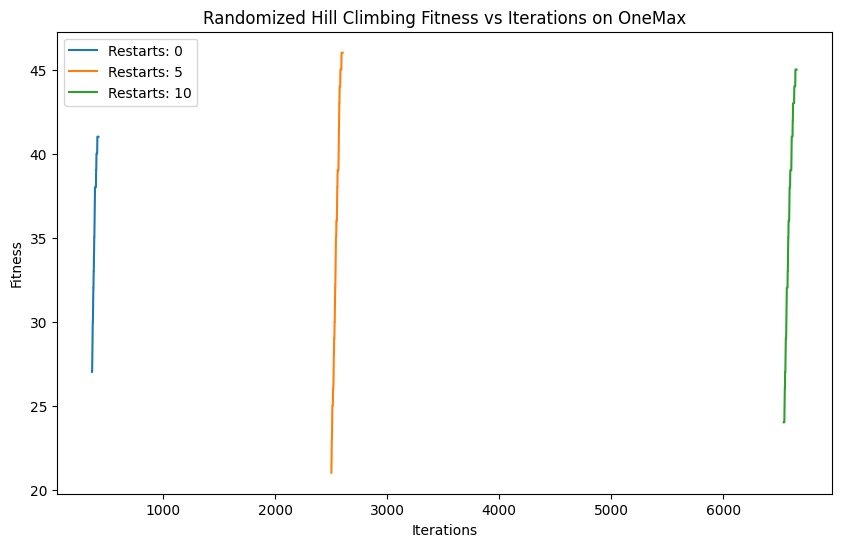
\includegraphics[width=\textwidth]{image/onemax/rhc.png}
        \caption{}
        \label{fig:onemaxrhc}
    \end{subfigure}
    \hfill
    \begin{subfigure}[b]{0.49\textwidth}
        \centering
        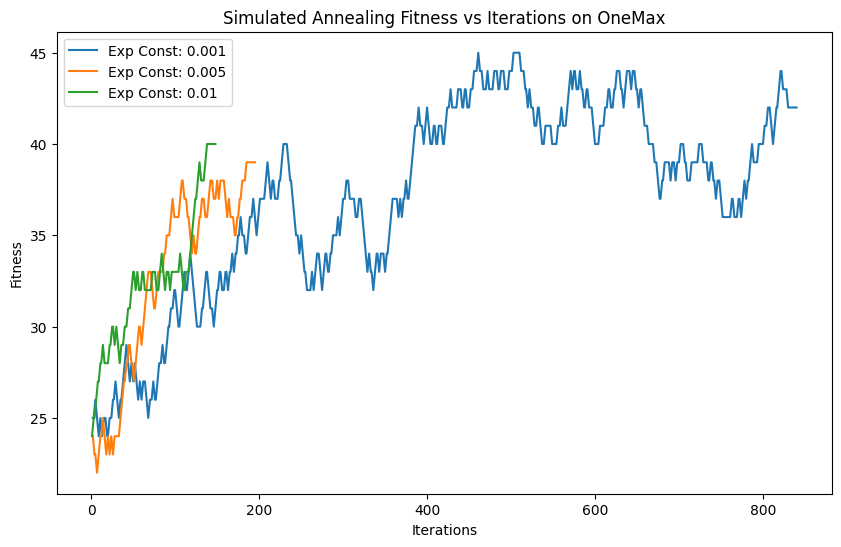
\includegraphics[width=\textwidth]{image/onemax/sa.png}
        \caption{}
        \label{fig:onemaxsa}
    \end{subfigure}
    \vskip\baselineskip
    \begin{subfigure}[b]{0.49\textwidth}
        \centering
        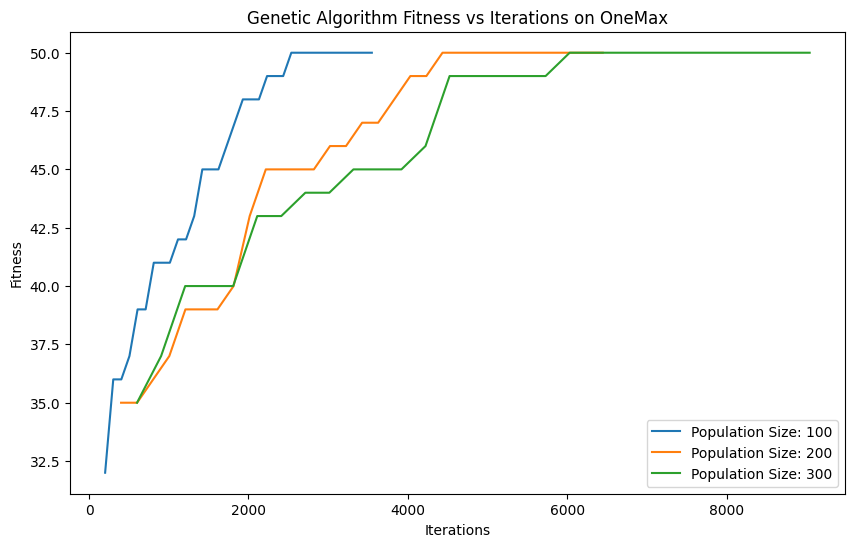
\includegraphics[width=\textwidth]{image/onemax/ga.png}
        \caption{}
        \label{fig:onemaxga}
    \end{subfigure}
    \hfill
    \begin{subfigure}[b]{0.49\textwidth}
        \centering
        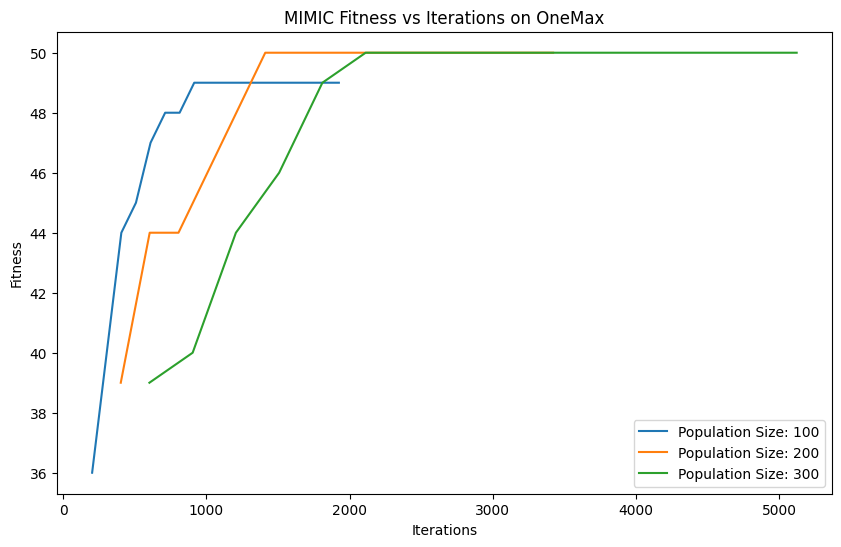
\includegraphics[width=\textwidth]{image/onemax/mimic.png}
        \caption{}
        \label{fig:onemaxmimic}
    \end{subfigure}
    \caption{Fitness vs. iterations for the OneMax using different randomized optimization algorithms: (a) RHC, (b) SA, (c) GA, and (d) MIMIC. The plots show the impact of varying key parameters—restarts for RHC, exponential cooling for SA, population sizes for GA, and population sizes for MIMIC—on the fitness progression over iterations.}
    \label{fig:onemaxgrid}
\end{figure*}

%flipflop
In the FlipFlop problem, where the objective is to maximize the number of alternating sequences of 1’s and 0’s in a binary string, the performance of the algorithms exhibits both similarities and differences compared to the OneMax problem. Genetic Algorithms (GA) and MIMIC continue to perform strongly, with GA achieving an average fitness of 48 for a population size of 300 and MIMIC closely matching with a fitness of 46.8 at the same population size (Table IV). This is because both GA and MIMIC are well-suited to explore the more rugged landscape of the FlipFlop problem, which includes more local optima than the smooth OneMax problem, as seen in Figures 2(c) and 2(d). In contrast, Randomized Hill Climbing (RHC) struggles significantly more with FlipFlop, achieving only 33.0 fitness without restarts, and improving marginally to 37.6 with 5 restarts, indicating that RHC's inability to effectively escape local optima is even more pronounced in this problem (Table IV, Figure 2(a)). Simulated Annealing (SA), although somewhat improved compared to OneMax, still suffers from inconsistencies in performance due to its probabilistic acceptance of worse solutions, with fitness values fluctuating between 41.2 and 43.0 depending on the cooling schedule (Table IV, Figure 2(b)). This fluctuation shows that while SA’s flexibility allows it to explore the more complex landscape, the inherent noise in its search process continues to prevent it from reliably reaching optimal solutions, especially when compared to the more structured approaches of GA and MIMIC. In summary, while GA and MIMIC remain highly effective for both OneMax and FlipFlop, the ruggedness of the FlipFlop landscape accentuates the limitations of RHC and SA, making them less competitive in this scenario.
\begin{table*}[h!]
    \centering
    \caption{FlipFlop Problem Results for RHC, SA, GA, and MIMIC with Different Hyperparameters}
    \begin{tabular}{|c|c|c|c|c|c|c|c|}
        \hline
        \textbf{Algorithm} & \textbf{Param} & \textbf{Run 1} & \textbf{Run 2} & \textbf{Run 3} & \textbf{Run 4} & \textbf{Average Fitness} & \textbf{Iterations} \\ \hline
        
        \textbf{RHC} & Restarts = 0 & 36.0 & 32.0 & 37.0 & 30.0 & 33.0 & 22 \\ \hline
        \textbf{RHC} & Restarts = 5 & 38.0 & 38.0 & 35.0 & 38.0 & 37.6 & 37 \\ \hline
        \textbf{RHC} & Restarts = 10 & 36.0 & 38.0 & 38.0 & 36.0 & 36.6 & 10 \\ \hline
        
        \textbf{SA} & ExpConst = 0.001 & 40.0 & 44.0 & 41.0 & 41.0 & 41.8 & 587 \\ \hline
        \textbf{SA} & ExpConst = 0.005 & 43.0 & 39.0 & 42.0 & 41.0 & 41.2 & 277 \\ \hline
        \textbf{SA} & ExpConst = 0.01 & 44.0 & 43.0 & 42.0 & 42.0 & 43.0 & 130 \\ \hline
        
        \textbf{GA} & PopSize = 100 & 46.0 & 39.0 & 42.0 & 46.0 & 43.8 & 46 \\ \hline
        \textbf{GA} & PopSize = 200 & 48.0 & 47.0 & 40.0 & 40.0 & 43.0 & 19 \\ \hline
        \textbf{GA} & PopSize = 300 & 39.0 & 48.0 & 42.0 & 46.0 & 43.0 & 62 \\ \hline
        
        \textbf{MIMIC} & PopSize = 100 & 43.0 & 41.0 & 42.0 & 45.0 & 42.8 & 16 \\ \hline
        \textbf{MIMIC} & PopSize = 200 & 45.0 & 47.0 & 44.0 & 47.0 & 45.6 & 18 \\ \hline
        \textbf{MIMIC} & PopSize = 300 & 46.0 & 46.0 & 47.0 & 48.0 & 46.8 & 18 \\ \hline
        
    \end{tabular}
    \label{tab:flipflop_results}
\end{table*}
\begin{figure*}[htbp]
    \centering
    \begin{subfigure}[b]{0.49\textwidth}
        \centering
        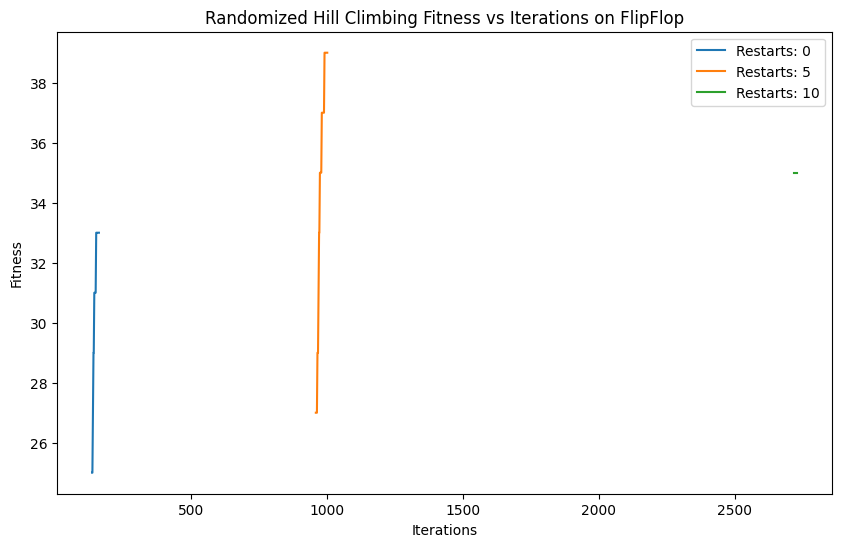
\includegraphics[width=\textwidth]{image/flipflop/rhc.png}
        \caption{}
        \label{fig:flipfloprhc}
    \end{subfigure}
    \hfill
    \begin{subfigure}[b]{0.49\textwidth}
        \centering
        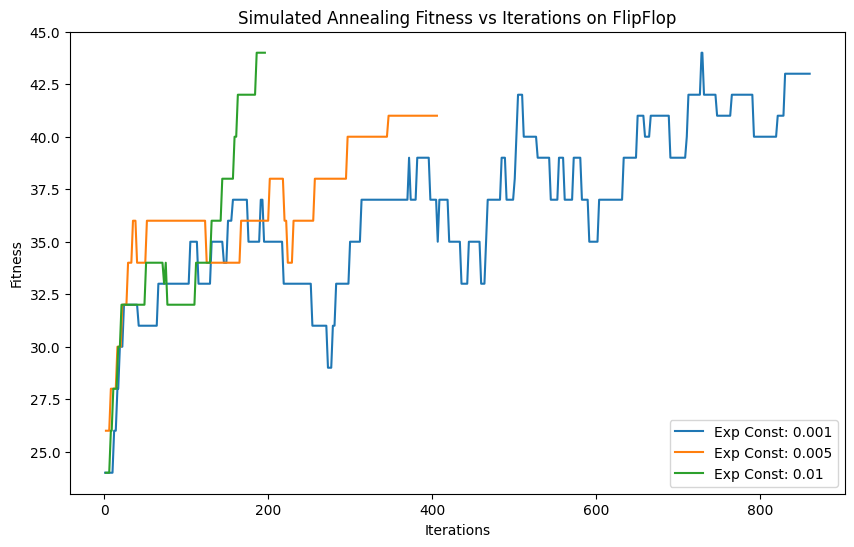
\includegraphics[width=\textwidth]{image/flipflop/sa.png}
        \caption{}
        \label{fig:flipflopsa}
    \end{subfigure}
    \vskip\baselineskip
    \begin{subfigure}[b]{0.49\textwidth}
        \centering
        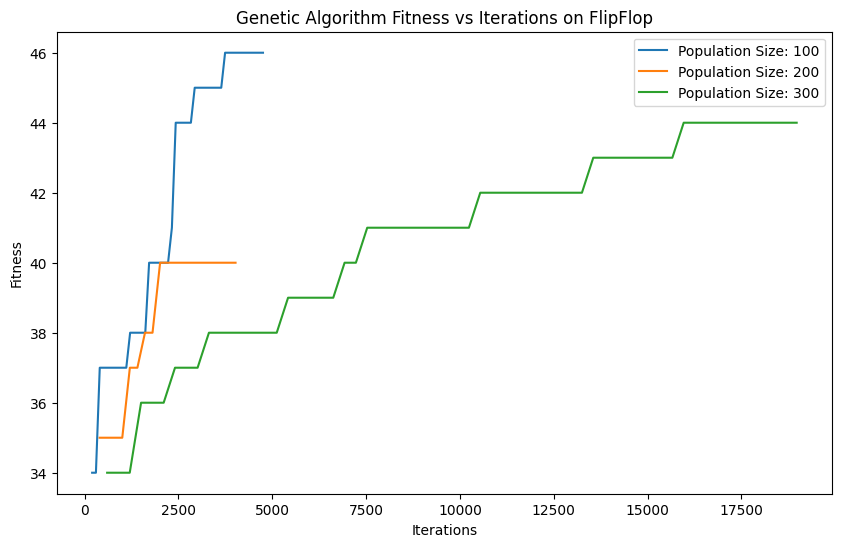
\includegraphics[width=\textwidth]{image/flipflop/ga.png}
        \caption{}
        \label{fig:flipflopga}
    \end{subfigure}
    \hfill
    \begin{subfigure}[b]{0.49\textwidth}
        \centering
        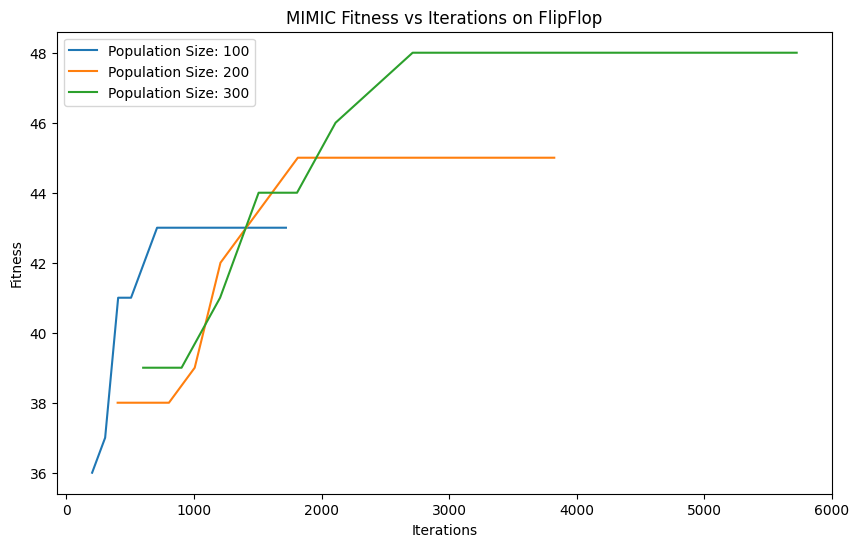
\includegraphics[width=\textwidth]{image/flipflop/mimic.png}
        \caption{}
        \label{fig:flipflopmimic}
    \end{subfigure}
    \caption{Fitness vs. iterations for the FlipFlop using different randomized optimization algorithms: (a) RHC, (b) SA, (c) GA, and (d) MIMIC. The plots show the impact of varying key parameters—restarts for RHC, exponential cooling for SA, population sizes for GA, and population sizes for MIMIC—on the fitness progression over iterations.}
    \label{fig:flipflopgrid}
\end{figure*}

%fourpeaks
In the FourPeaks problem, where the goal is to balance between finding both long runs of 1's and 0's in a binary string, the performance of the algorithms highlights the challenge of navigating a more complex landscape with multiple local optima. Genetic Algorithms (GA) and MIMIC again perform well, with GA achieving a high average fitness of 85.8 for a population size of 300 (Table V), and MIMIC close behind at 68.4 with the same population size. As seen in Figures 3(c) and 3(d), both algorithms quickly converge to near-optimal solutions, but GA is notably faster in reaching higher fitness values, demonstrating its advantage in balancing exploration and exploitation for this problem's complex landscape. In contrast, Randomized Hill Climbing (RHC) struggles significantly, achieving a maximum fitness of only 6.0 with 10 restarts (Table V, Figure 3(a)), as it cannot effectively escape local optima in the FourPeaks landscape, where more global exploration is crucial. Simulated Annealing (SA), while showing better results than RHC, has highly variable performance depending on the cooling schedule, with the best average fitness of 39.8 when using an exponential constant of 0.01 (Table V, Figure 3(b)). SA's ability to accept worse solutions helps in this problem, but its stochastic nature introduces instability in performance, making it less reliable than GA or MIMIC. Compared to the FlipFlop problem, both RHC and SA struggle more here, reflecting the added complexity and local minima present in FourPeaks.
\begin{table*}[h!]
    \centering
    \caption{FourPeaks Problem Results for RHC, SA, GA, and MIMIC with Different Hyperparameters}
    \begin{tabular}{|c|c|c|c|c|c|c|c|}
        \hline
        \textbf{Algorithm} & \textbf{Param} & \textbf{Run 1} & \textbf{Run 2} & \textbf{Run 3} & \textbf{Run 4} & \textbf{Average Fitness} & \textbf{Iterations} \\ \hline
        
        \textbf{RHC} & Restarts = 0 & 0.0 & 1.0 & 6.0 & 4.0 & 2.2 & 10 \\ \hline
        \textbf{RHC} & Restarts = 5 & 6.0 & 6.0 & 7.0 & 7.0 & 5.8 & 10 \\ \hline
        \textbf{RHC} & Restarts = 10 & 7.0 & 11.0 & 4.0 & 4.0 & 6.0 & 10 \\ \hline
        
        \textbf{SA} & ExpConst = 0.001 & 18.0 & 26.0 & 40.0 & 30.0 & 29.0 & 941 \\ \hline
        \textbf{SA} & ExpConst = 0.005 & 38.0 & 43.0 & 22.0 & 29.0 & 31.4 & 645 \\ \hline
        \textbf{SA} & ExpConst = 0.01 & 31.0 & 36.0 & 25.0 & 31.0 & 39.8 & 538 \\ \hline
        
        \textbf{GA} & PopSize = 100 & 30.0 & 21.0 & 25.0 & 32.0 & 35.4 & 37 \\ \hline
        \textbf{GA} & PopSize = 200 & 76.0 & 73.0 & 69.0 & 34.0 & 66.4 & 48 \\ \hline
        \textbf{GA} & PopSize = 300 & 87.0 & 86.0 & 79.0 & 91.0 & 86.8 & 57 \\ \hline
        
        \textbf{MIMIC} & PopSize = 100 & 63.0 & 13.0 & 60.0 & 15.0 & 34.2 & 26 \\ \hline
        \textbf{MIMIC} & PopSize = 200 & 78.0 & 19.0 & 71.0 & 73.0 & 60.2 & 28 \\ \hline
        \textbf{MIMIC} & PopSize = 300 & 83.0 & 21.0 & 76.0 & 71.0 & 68.4 & 41 \\ \hline
        
    \end{tabular}
    \label{tab:fourpeaks_results}
\end{table*}
\begin{figure*}[htbp]
    \centering
    \begin{subfigure}[b]{0.49\textwidth}
        \centering
        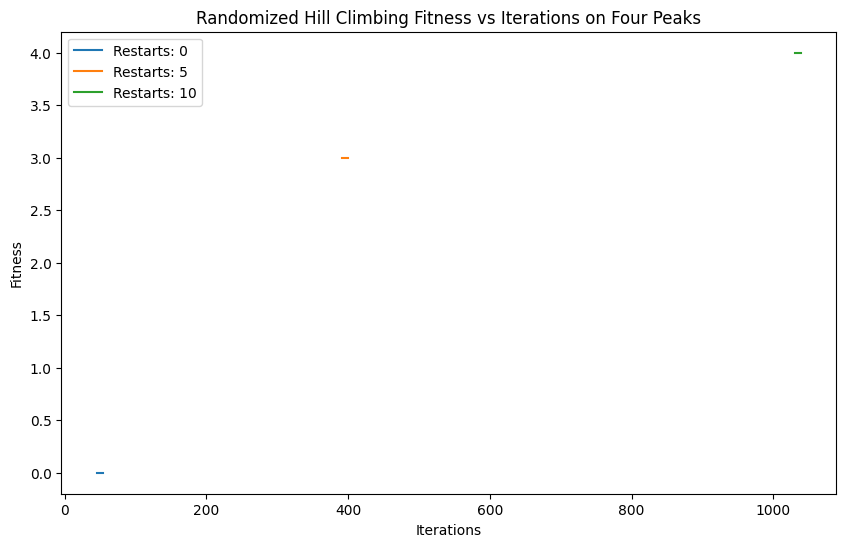
\includegraphics[width=\textwidth]{image/fourpeak/rhc.png}
        \caption{}
        \label{fig:fourpeakrhc}
    \end{subfigure}
    \hfill
    \begin{subfigure}[b]{0.49\textwidth}
        \centering
        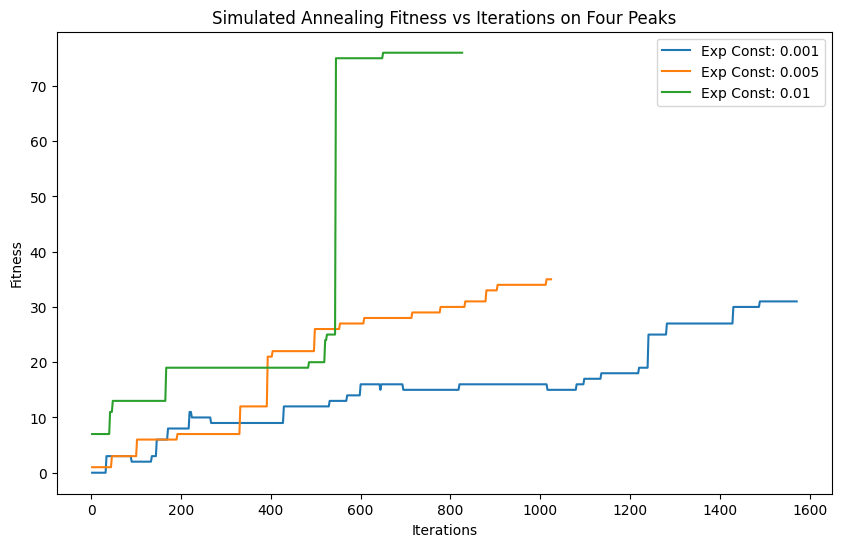
\includegraphics[width=\textwidth]{image/fourpeak/sa.png}
        \caption{}
        \label{fig:fourpeaksa}
    \end{subfigure}
    \vskip\baselineskip
    \begin{subfigure}[b]{0.49\textwidth}
        \centering
        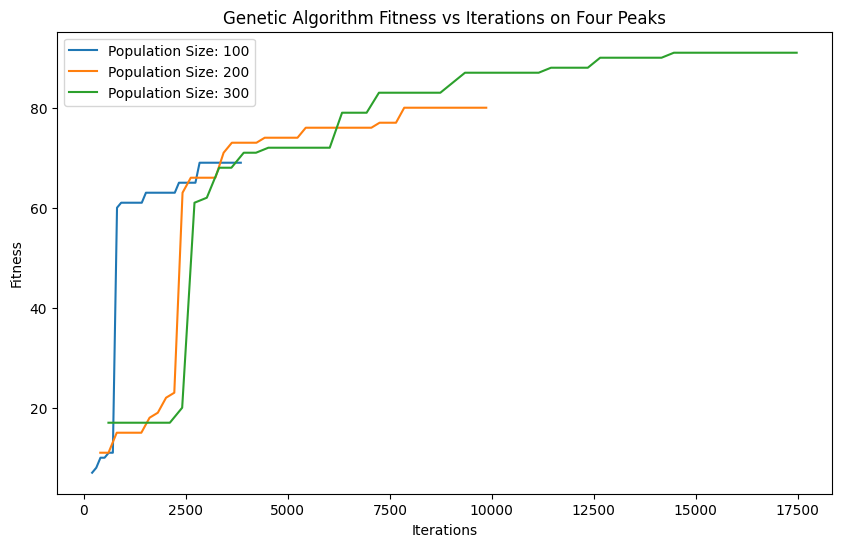
\includegraphics[width=\textwidth]{image/fourpeak/ga.png}
        \caption{}
        \label{fig:fourpeakga}
    \end{subfigure}
    \hfill
    \begin{subfigure}[b]{0.49\textwidth}
        \centering
        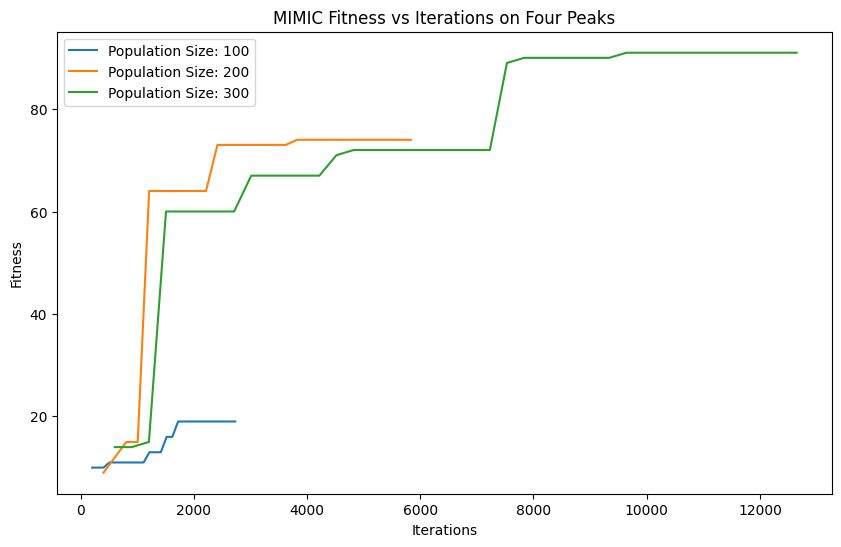
\includegraphics[width=\textwidth]{image/fourpeak/mimic.png}
        \caption{}
        \label{fig:fourpeakmimic}
    \end{subfigure}
    \caption{Fitness vs. iterations for the FourPeaks using different randomized optimization algorithms: (a) RHC, (b) SA, (c) GA, and (d) MIMIC. The plots show the impact of varying key parameters—restarts for RHC, exponential cooling for SA, population sizes for GA, and population sizes for MIMIC—on the fitness progression over iterations.}
    \label{fig:fourpeakgrid}
\end{figure*}

%sixpeaks
In the SixPeaks problem, where the task is to optimize both peaks of 0’s and 1’s while rewarding strings that achieve long runs, we observe varying performance across algorithms, particularly highlighting the challenges of balancing exploration and exploitation in this more rugged search space. Genetic Algorithms (GA) and MIMIC again show strong results, with GA reaching an average fitness of 89.2 with a population size of 200 and MIMIC achieving 75.0 with a population size of 300 (Table VI). GA’s ability to reach high fitness efficiently, seen in Figure 4(c), reflects its success in quickly navigating this problem’s dual-peak structure, where the balance between exploration and exploitation is critical. MIMIC also demonstrates strong performance, as shown in Figure 4(d), converging steadily with different population sizes, though at a slightly slower pace than GA. Meanwhile, Randomized Hill Climbing (RHC) struggles even more in the SixPeaks problem compared to previous benchmarks, with fitness values only reaching an average of 9.4 with 10 restarts, highlighting its severe limitations in overcoming the local optima present in the landscape (Table VI, Figure 4(a)). Simulated Annealing (SA), with its inherent flexibility to escape local minima, performs relatively better, reaching an average fitness of 37.0 at the best cooling schedule (ExpConst = 0.01), but still lags behind both GA and MIMIC, as seen in Figure 4(b). Compared to the FourPeaks problem, SA’s performance improves marginally in SixPeaks due to the higher level of exploration required, but it remains less efficient overall. This analysis demonstrates that while GA and MIMIC maintain their dominance, the increased complexity of the SixPeaks landscape intensifies the shortcomings of RHC and exposes the need for more sophisticated exploration mechanisms in SA
\begin{table*}[h!]
    \centering
    \caption{SixPeaks Problem Results for RHC, SA, GA, and MIMIC with Different Hyperparameters}
    \begin{tabular}{|c|c|c|c|c|c|c|c|}
        \hline
        \textbf{Algorithm} & \textbf{Param} & \textbf{Run 1} & \textbf{Run 2} & \textbf{Run 3} & \textbf{Run 4} & \textbf{Average Fitness} & \textbf{Iterations} \\ \hline
        
        \textbf{RHC} & Restarts = 0 & 2.0 & 1.0 & 10.0 & 1.0 & 3.2 & 10 \\ \hline
        \textbf{RHC} & Restarts = 5 & 6.0 & 6.0 & 8.0 & 7.0 & 6.6 & 21 \\ \hline
        \textbf{RHC} & Restarts = 10 & 12.0 & 6.0 & 10.0 & 8.0 & 9.4 & 17 \\ \hline
        
        \textbf{SA} & ExpConst = 0.001 & 22.0 & 19.0 & 41.0 & 31.0 & 28.0 & 1000 \\ \hline
        \textbf{SA} & ExpConst = 0.005 & 34.0 & 24.0 & 35.0 & 35.0 & 31.6 & 869 \\ \hline
        \textbf{SA} & ExpConst = 0.01 & 33.0 & 42.0 & 35.0 & 34.0 & 37.0 & 966 \\ \hline
        
        \textbf{GA} & PopSize = 100 & 15.0 & 50.0 & 19.0 & 76.0 & 40.0 & 28 \\ \hline
        \textbf{GA} & PopSize = 200 & 91.0 & 91.0 & 87.0 & 91.0 & 89.2 & 21 \\ \hline
        \textbf{GA} & PopSize = 300 & 66.0 & 75.0 & 84.0 & 76.0 & 73.8 & 26 \\ \hline
        
        \textbf{MIMIC} & PopSize = 100 & 65.0 & 16.0 & 18.0 & 23.0 & 26.4 & 11 \\ \hline
        \textbf{MIMIC} & PopSize = 200 & 63.0 & 76.0 & 83.0 & 73.0 & 73.4 & 16 \\ \hline
        \textbf{MIMIC} & PopSize = 300 & 73.0 & 71.0 & 77.0 & 82.0 & 75.0 & 24 \\ \hline
        
    \end{tabular}
    \label{tab:sixpeaks_results}
\end{table*}
\begin{figure*}[htbp]
    \centering
    \begin{subfigure}[b]{0.49\textwidth}
        \centering
        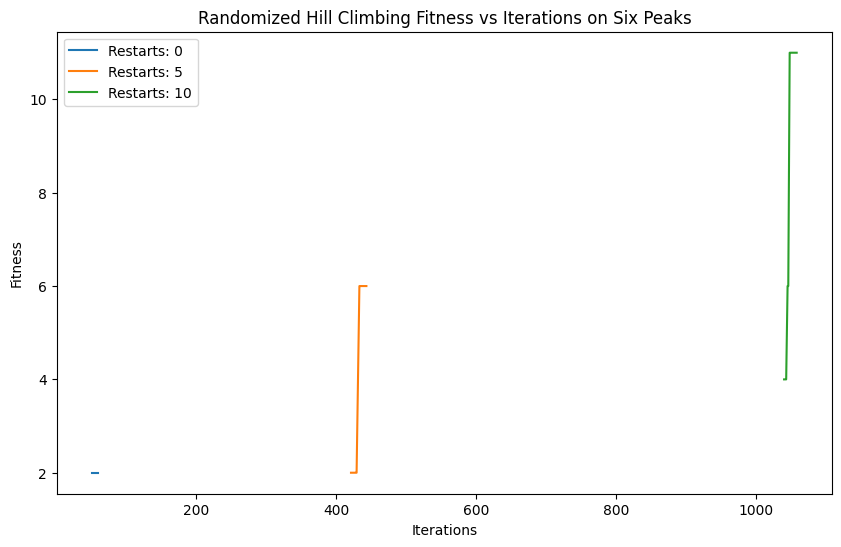
\includegraphics[width=\textwidth]{image/sixpeak/rhc.png}
        \caption{}
        \label{fig:sixpeakrhc}
    \end{subfigure}
    \hfill
    \begin{subfigure}[b]{0.49\textwidth}
        \centering
        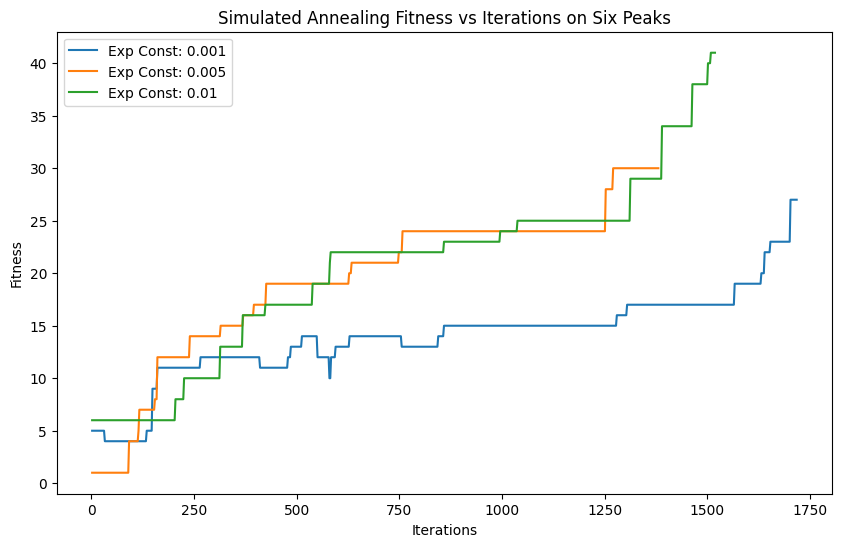
\includegraphics[width=\textwidth]{image/sixpeak/sa.png}
        \caption{}
        \label{fig:sixpeaksa}
    \end{subfigure}
    \vskip\baselineskip
    \begin{subfigure}[b]{0.49\textwidth}
        \centering
        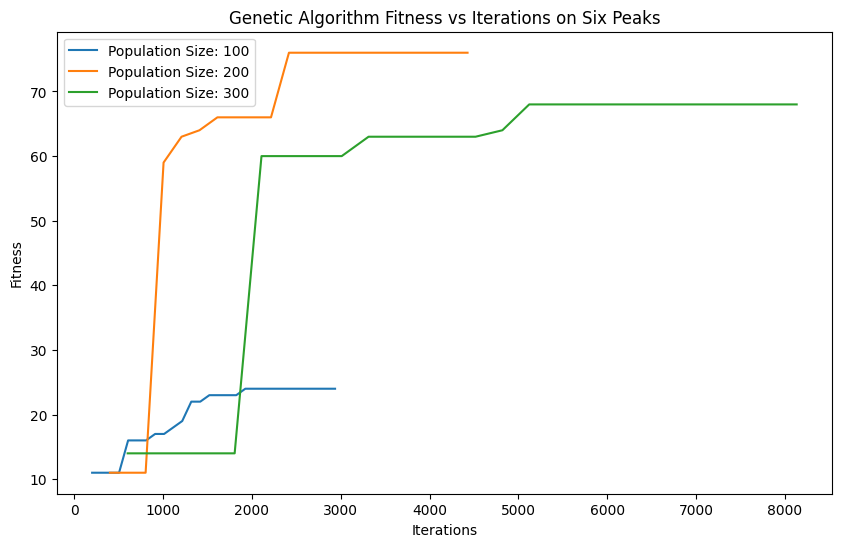
\includegraphics[width=\textwidth]{image/sixpeak/ga.png}
        \caption{}
        \label{fig:sixpeakga}
    \end{subfigure}
    \hfill
    \begin{subfigure}[b]{0.49\textwidth}
        \centering
        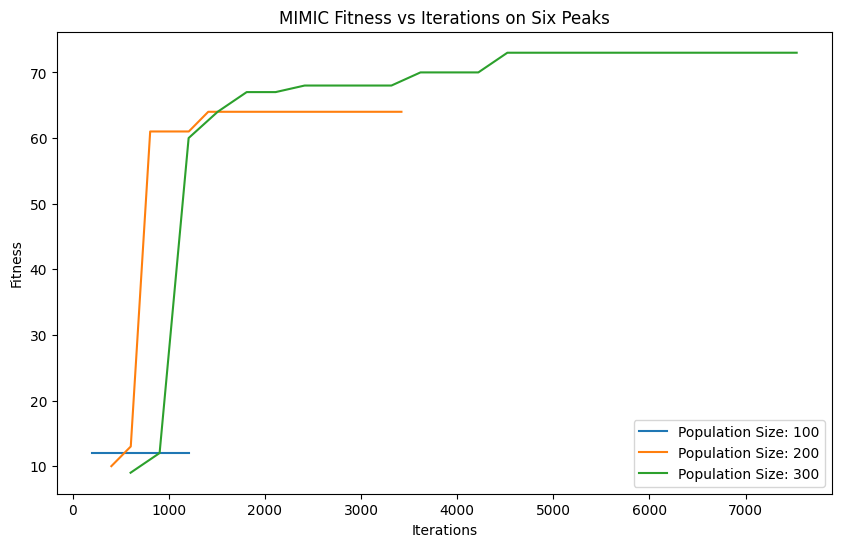
\includegraphics[width=\textwidth]{image/sixpeak/mimic.png}
        \caption{}
        \label{fig:sixpeakmimic}
    \end{subfigure}
    \caption{Fitness vs. iterations for the SixPeaks using different randomized optimization algorithms: (a) RHC, (b) SA, (c) GA, and (d) MIMIC. The plots show the impact of varying key parameters—restarts for RHC, exponential cooling for SA, population sizes for GA, and population sizes for MIMIC—on the fitness progression over iterations.}
    \label{fig:sixpeakgrid}
\end{figure*}

%Continuous Peaks
In the ContinuousPeaks problem, where the goal is to balance between long sequences of 0’s and 1’s while providing a bonus for achieving long runs of both, the results reflect the varying effectiveness of each algorithm in navigating this more complex landscape. Genetic Algorithms (GA) and MIMIC continue to excel, with GA achieving an average fitness of 82.4 for a population size of 200 and MIMIC reaching 80.8 with a population size of 300 (Table VII). GA’s efficiency in this problem, as seen in Figure 5(c), is due to its ability to exploit the structured peaks in the search space, allowing for rapid convergence to high-quality solutions. MIMIC also performs well, steadily improving with larger population sizes (Figure 5(d)), although it converges slightly more slowly compared to GA. Randomized Hill Climbing (RHC) shows poor performance once again, with an average fitness of only 23.8 even with 10 restarts, underscoring its limitations in escaping local optima in this more rugged landscape (Table VII, Figure 5(a)). Simulated Annealing (SA), however, performs much better in this problem compared to previous benchmarks, achieving an average fitness of 77.2 with an exponential constant of 0.001, likely due to the problem’s more defined peaks, which align well with SA's probabilistic exploration mechanism (Table VII, Figure 5(b)). Despite this, SA still struggles with convergence speed, as seen in the large number of iterations required compared to GA and MIMIC. Overall, the results show that while GA and MIMIC remain the top performers, SA demonstrates stronger results in ContinuousPeaks due to its ability to navigate the problem’s well-defined peaks, though at the cost of computational efficiency.
\begin{table*}[h!]
    \centering
    \caption{ContinuousPeaks Problem Results for RHC, SA, GA, and MIMIC with Different Hyperparameters}
    \begin{tabular}{|c|c|c|c|c|c|c|c|}
        \hline
        \textbf{Algorithm} & \textbf{Param} & \textbf{Run 1} & \textbf{Run 2} & \textbf{Run 3} & \textbf{Run 4} & \textbf{Average Fitness} & \textbf{Iterations} \\ \hline
        
        \textbf{RHC} & Restarts = 0 & 8.0 & 13.0 & 6.0 & 8.0 & 8.6 & 16 \\ \hline
        \textbf{RHC} & Restarts = 5 & 7.0 & 16.0 & 9.0 & 8.0 & 9.6 & 10 \\ \hline
        \textbf{RHC} & Restarts = 10 & 14.0 & 13.0 & 12.0 & 69.0 & 23.8 & 24 \\ \hline
        
        \textbf{SA} & ExpConst = 0.001 & 82.0 & 71.0 & 88.0 & 75.0 & 77.2 & 712 \\ \hline
        \textbf{SA} & ExpConst = 0.005 & 82.0 & 41.0 & 43.0 & 77.0 & 64.6 & 222 \\ \hline
        \textbf{SA} & ExpConst = 0.01 & 81.0 & 85.0 & 43.0 & 71.0 & 71.8 & 483 \\ \hline
        
        \textbf{GA} & PopSize = 100 & 69.0 & 68.0 & 80.0 & 68.0 & 71.0 & 32 \\ \hline
        \textbf{GA} & PopSize = 200 & 83.0 & 83.0 & 68.0 & 88.0 & 82.4 & 43 \\ \hline
        \textbf{GA} & PopSize = 300 & 84.0 & 87.0 & 75.0 & 86.0 & 81.6 & 29 \\ \hline
        
        \textbf{MIMIC} & PopSize = 100 & 77.0 & 65.0 & 69.0 & 66.0 & 68.2 & 15 \\ \hline
        \textbf{MIMIC} & PopSize = 200 & 77.0 & 75.0 & 76.0 & 74.0 & 74.4 & 18 \\ \hline
        \textbf{MIMIC} & PopSize = 300 & 87.0 & 76.0 & 82.0 & 78.0 & 80.8 & 22 \\ \hline
        
    \end{tabular}
    \label{tab:continuouspeaks_results}
\end{table*}
\begin{figure*}[htbp]
    \centering
    \begin{subfigure}[b]{0.49\textwidth}
        \centering
        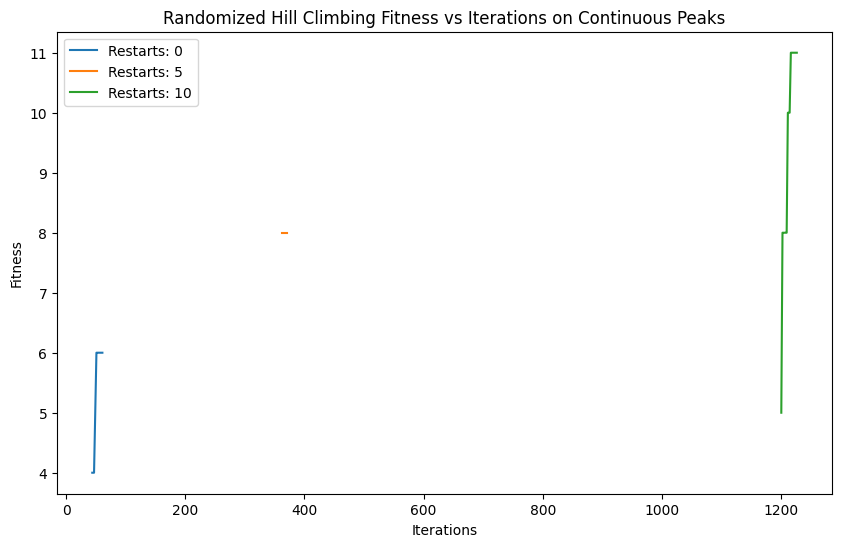
\includegraphics[width=\textwidth]{image/continuouspeak/rhc.png}
        \caption{}
        \label{fig:continuouspeakrhc}
    \end{subfigure}
    \hfill
    \begin{subfigure}[b]{0.49\textwidth}
        \centering
        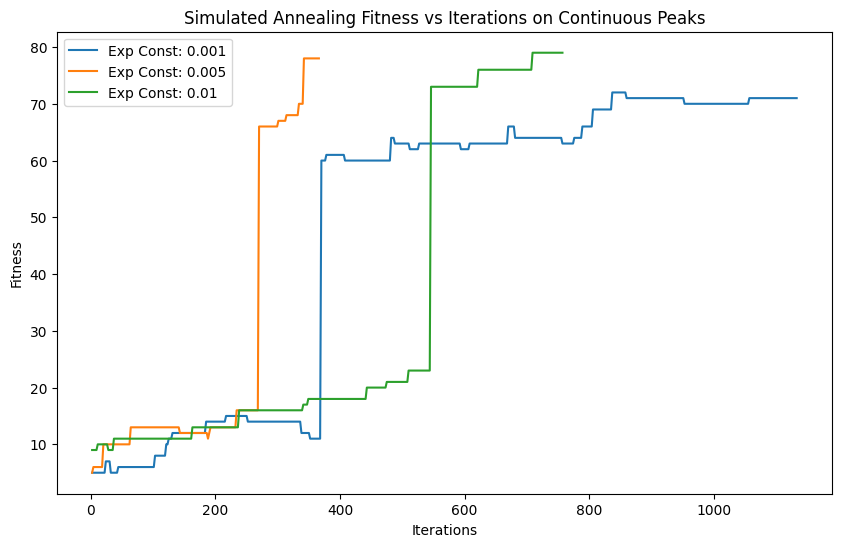
\includegraphics[width=\textwidth]{image/continuouspeak/sa.png}
        \caption{}
        \label{fig:continuouspeaksa}
    \end{subfigure}
    \vskip\baselineskip
    \begin{subfigure}[b]{0.49\textwidth}
        \centering
        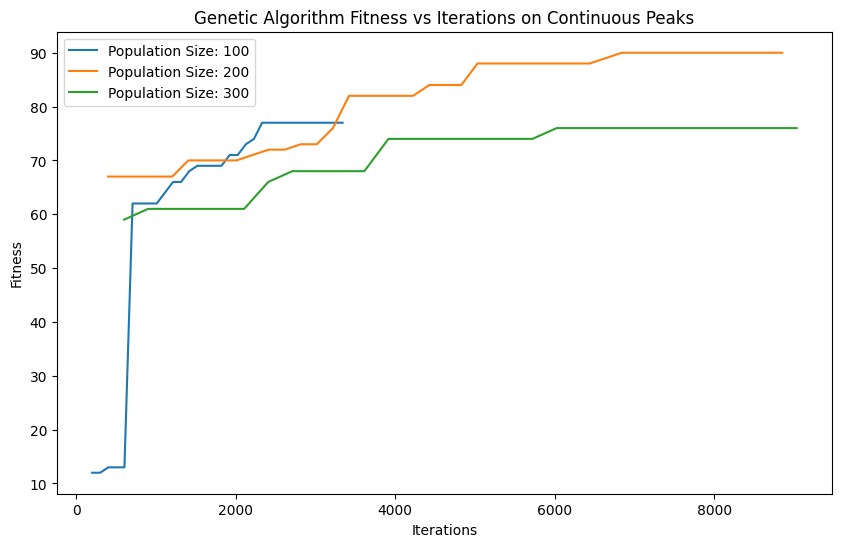
\includegraphics[width=\textwidth]{image/continuouspeak/ga.png}
        \caption{}
        \label{fig:continuouspeakga}
    \end{subfigure}
    \hfill
    \begin{subfigure}[b]{0.49\textwidth}
        \centering
        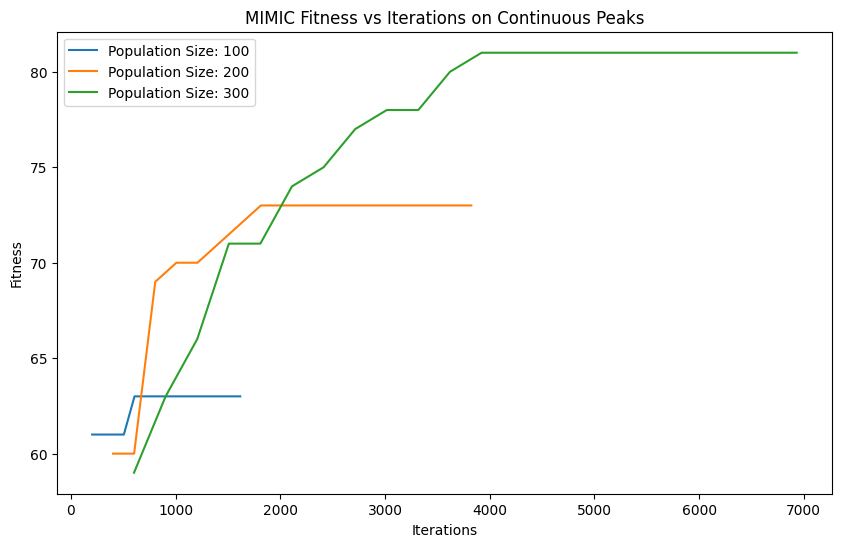
\includegraphics[width=\textwidth]{image/continuouspeak/mimic.png}
        \caption{}
        \label{fig:continuouspeakmimic}
    \end{subfigure}
    \caption{Fitness vs. iterations for the ContinuousPeaks using different randomized optimization algorithms: (a) RHC, (b) SA, (c) GA, and (d) MIMIC. The plots show the impact of varying key parameters—restarts for RHC, exponential cooling for SA, population sizes for GA, and population sizes for MIMIC—on the fitness progression over iterations.}
    \label{fig:continuouspeakgrid}
\end{figure*}

\subsection{Permutation Problems}

%tsp
In the Traveling Salesman Problem (TSP), where the goal is to find the shortest possible route through a set of cities, the performance of the algorithms reflects the challenge of navigating a complex, highly constrained search space. Randomized Hill Climbing (RHC) performs poorly, achieving an average fitness of only 11.52 with 10 restarts, showing its limitations in escaping local optima in this permutation-based problem (Table VIII, Figure 6(a)). Simulated Annealing (SA) performs better but still struggles with high variability, achieving its best fitness of 13.91 at an exponential constant of 0.001 (Table VIII). However, its fitness fluctuates significantly, as seen in Figure 6(b), indicating that the probabilistic acceptance of worse solutions leads to instability in finding optimal routes. In contrast, Genetic Algorithms (GA) show a more stable yet slower convergence pattern, with an average fitness of 8.80 for a population size of 100 (Table VIII). As shown in Figure 6(c), GA's crossover and mutation operators help it explore the TSP's complex solution space more systematically, but it converges slowly. MIMIC, on the other hand, achieves the highest average fitness of 18.47 with a population size of 100 (Table VIII), reflecting its ability to effectively sample from promising regions of the solution space using its probabilistic model. Figure 6(d) demonstrates that MIMIC converges faster than GA, particularly for smaller population sizes, making it more efficient in solving the TSP, though it also shows a plateau effect in larger populations.
\begin{table*}[h!]
    \centering
    \caption{Traveling Salesman Problem Results for RHC, SA, GA, and MIMIC with Different Hyperparameters}
    \begin{tabular}{|c|c|c|c|c|c|c|c|}
        \hline
        \textbf{Algorithm} & \textbf{Param} & \textbf{Run 1} & \textbf{Run 2} & \textbf{Run 3} & \textbf{Run 4} & \textbf{Average Fitness} & \textbf{Iterations} \\ \hline
        
        \textbf{RHC} & Restarts = 0 & 12.83 & 15.88 & 15.15 & 17.69 & 16.05 & 21 \\ \hline
        \textbf{RHC} & Restarts = 5 & 12.20 & 14.70 & 13.83 & 12.40 & 13.78 & 63 \\ \hline
        \textbf{RHC} & Restarts = 10 & 12.87 & 11.63 & 11.18 & 10.26 & 11.52 & 66 \\ \hline
        
        \textbf{SA} & ExpConst = 0.001 & 15.20 & 12.73 & 12.88 & 14.75 & 13.91 & 761 \\ \hline
        \textbf{SA} & ExpConst = 0.005 & 12.94 & 11.03 & 14.44 & 13.57 & 13.40 & 333 \\ \hline
        \textbf{SA} & ExpConst = 0.01 & 14.30 & 13.90 & 12.79 & 13.71 & 13.52 & 191 \\ \hline
        
        \textbf{GA} & PopSize = 100 & 8.35 & 9.20 & 8.95 & 8.72 & 8.80 & 91 \\ \hline
        \textbf{GA} & PopSize = 200 & 7.27 & 6.05 & 7.61 & 6.23 & 6.91 & 119 \\ \hline
        \textbf{GA} & PopSize = 300 & 9.28 & 5.70 & 5.30 & 5.16 & 6.29 & 94 \\ \hline
        
        \textbf{MIMIC} & PopSize = 100 & 19.83 & 18.67 & 18.37 & 17.44 & 18.47 & 11 \\ \hline
        \textbf{MIMIC} & PopSize = 200 & 18.15 & 13.47 & 14.51 & 16.92 & 15.90 & 14 \\ \hline
        \textbf{MIMIC} & PopSize = 300 & 10.75 & 11.46 & 14.56 & 16.75 & 13.31 & 22 \\ \hline
        
    \end{tabular}
    \label{tab:tsp_results}
\end{table*}
\begin{figure*}[htbp]
    \centering
    \begin{subfigure}[b]{0.49\textwidth}
        \centering
        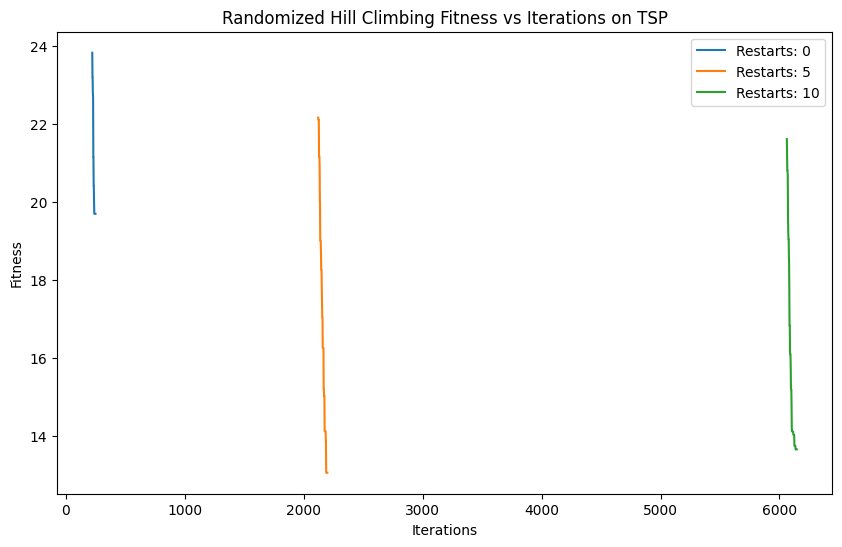
\includegraphics[width=\textwidth]{image/tsp/rhc.png}
        \caption{}
        \label{fig:tsprhc}
    \end{subfigure}
    \hfill
    \begin{subfigure}[b]{0.49\textwidth}
        \centering
        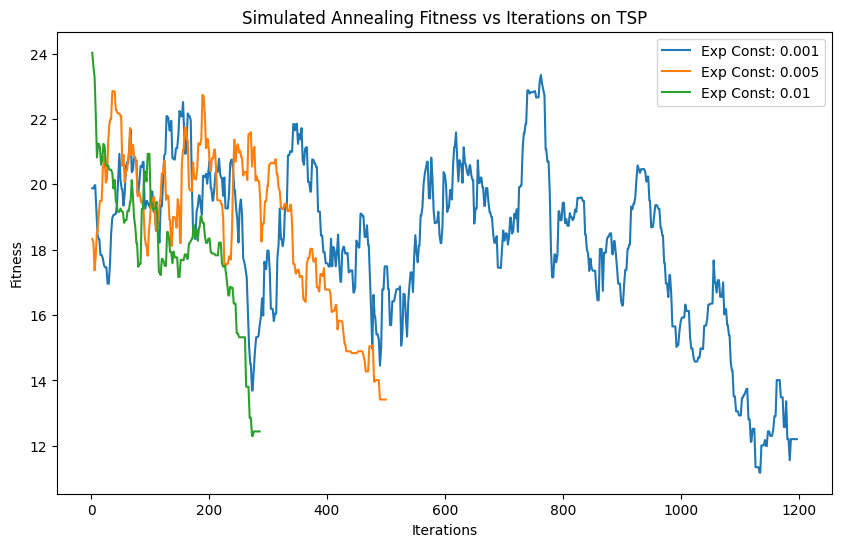
\includegraphics[width=\textwidth]{image/tsp/sa.png}
        \caption{}
        \label{fig:tspsa}
    \end{subfigure}
    \vskip\baselineskip
    \begin{subfigure}[b]{0.49\textwidth}
        \centering
        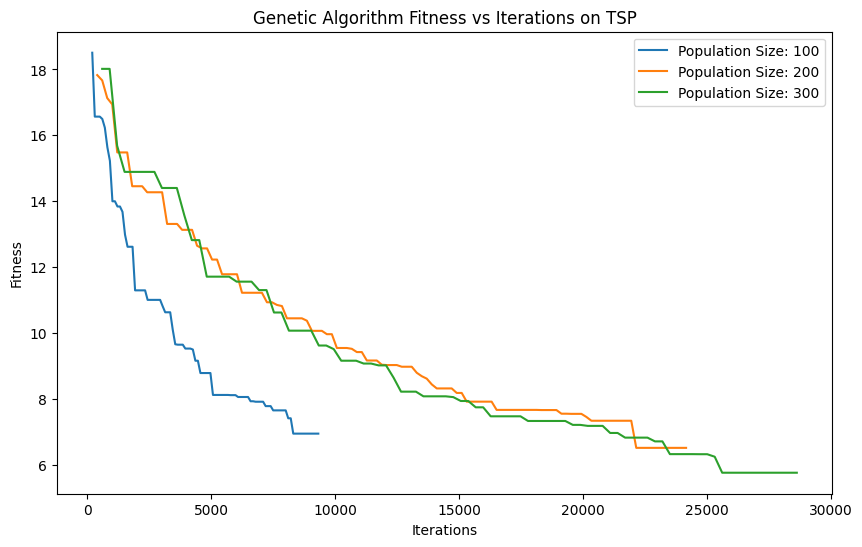
\includegraphics[width=\textwidth]{image/tsp/ga.png}
        \caption{}
        \label{fig:tspga}
    \end{subfigure}
    \hfill
    \begin{subfigure}[b]{0.49\textwidth}
        \centering
        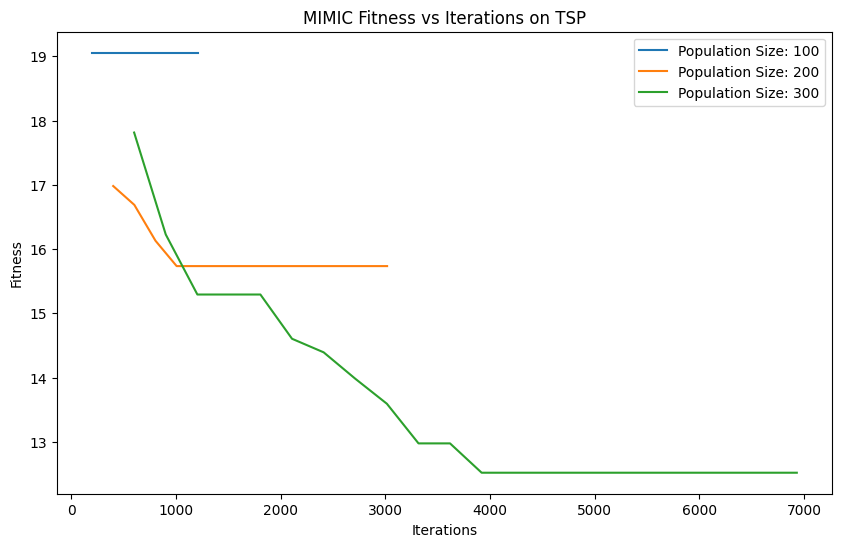
\includegraphics[width=\textwidth]{image/tsp/mimic.png}
        \caption{}
        \label{fig:tspmimic}
    \end{subfigure}
    \caption{Fitness vs. iterations for the Traveling Salesman Problem using different randomized optimization algorithms: (a) RHC, (b) SA, (c) GA, and (d) MIMIC. The plots show the impact of varying key parameters—restarts for RHC, exponential cooling for SA, population sizes for GA, and population sizes for MIMIC—on the fitness progression over iterations.}
    \label{fig:tspgrid}
\end{figure*}

%queens
In the Queens problem, where the objective is to place queens on a chessboard such that no two queens threaten each other, the results show that all algorithms perform significantly better than in previous permutation problems, reflecting the structured nature of the solution space. MIMIC performs best, with an average fitness of 95.4 for a population size of 300, quickly converging to near-optimal solutions (Table IX, Figure 7(d)). This highlights MIMIC’s strong ability to capture and exploit dependencies between variables in the Queens problem. Genetic Algorithms (GA) also perform well, achieving an average fitness of 90.1 with a population size of 100, though it takes longer to converge compared to MIMIC (Figure 7(c)). Simulated Annealing (SA) shows improved performance here compared to the Traveling Salesman Problem (TSP), with an average fitness of 90.6 at an exponential constant of 0.01, although its convergence is less stable, as shown in Figure 7(b). The probabilistic acceptance of worse solutions helps SA escape local optima, but it introduces variability, making it less reliable than GA and MIMIC in finding the optimal solution. Randomized Hill Climbing (RHC) performs reasonably well for a local search algorithm, reaching an average fitness of 85.6 with 5 restarts, but it still lags behind the other methods, as it struggles to maintain global exploration (Table IX, Figure 7(a)). 
\begin{table*}[h!]
    \centering
    \caption{Queens Problem Results for RHC, SA, GA, and MIMIC with Different Hyperparameters}
    \begin{tabular}{|c|c|c|c|c|c|c|c|}
        \hline
        \textbf{Algorithm} & \textbf{Param} & \textbf{Run 1} & \textbf{Run 2} & \textbf{Run 3} & \textbf{Run 4} & \textbf{Average Fitness} & \textbf{Iterations} \\ \hline
        
        \textbf{RHC} & Restarts = 0 & 84.0 & 80.0 & 85.0 & 78.0 & 81.4 & 22 \\ \hline
        \textbf{RHC} & Restarts = 5 & 86.0 & 86.0 & 83.0 & 86.0 & 85.6 & 37 \\ \hline
        \textbf{RHC} & Restarts = 10 & 84.0 & 86.0 & 86.0 & 84.0 & 85.0 & 10 \\ \hline
        
        \textbf{SA} & ExpConst = 0.001 & 88.0 & 92.0 & 89.0 & 89.0 & 89.8 & 587 \\ \hline
        \textbf{SA} & ExpConst = 0.005 & 91.0 & 87.0 & 90.0 & 89.0 & 89.2 & 277 \\ \hline
        \textbf{SA} & ExpConst = 0.01 & 92.0 & 91.0 & 90.0 & 90.0 & 90.6 & 130 \\ \hline
        
        \textbf{GA} & PopSize = 100 & 95.0 & 89.0 & 93.0 & 87.0 & 91.0 & 12 \\ \hline
        \textbf{GA} & PopSize = 200 & 89.0 & 85.0 & 86.0 & 88.0 & 86.8 & 13 \\ \hline
        \textbf{GA} & PopSize = 300 & 93.0 & 94.0 & 88.0 & 87.0 & 91.0 & 50 \\ \hline
        
        \textbf{MIMIC} & PopSize = 100 & 92.0 & 91.0 & 93.0 & 91.0 & 91.4 & 16 \\ \hline
        \textbf{MIMIC} & PopSize = 200 & 95.0 & 95.0 & 92.0 & 94.0 & 94.2 & 17 \\ \hline
        \textbf{MIMIC} & PopSize = 300 & 95.0 & 96.0 & 96.0 & 95.0 & 95.4 & 17 \\ \hline
        
    \end{tabular}
    \label{tab:queens_results}
\end{table*}
\begin{figure*}[htbp]
    \centering
    \begin{subfigure}[b]{0.49\textwidth}
        \centering
        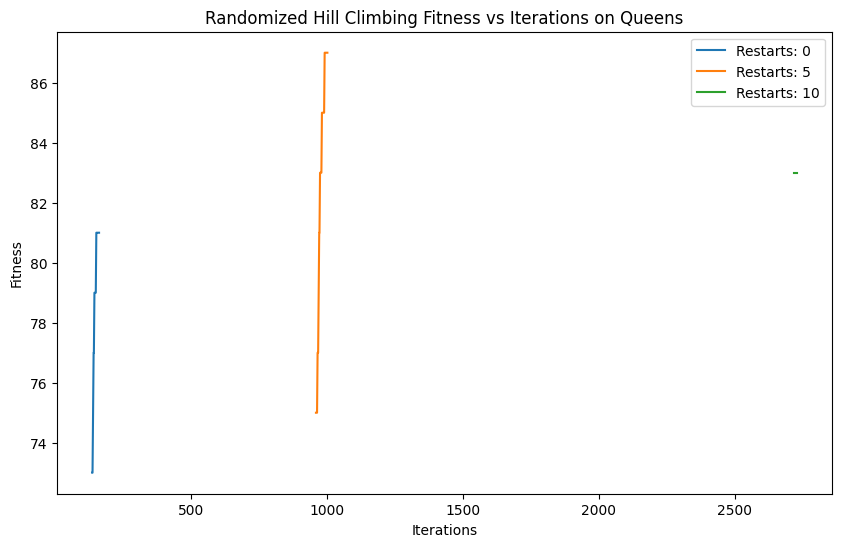
\includegraphics[width=\textwidth]{image/queens/rhc.png}
        \caption{}
        \label{fig:queensrhc}
    \end{subfigure}
    \hfill
    \begin{subfigure}[b]{0.49\textwidth}
        \centering
        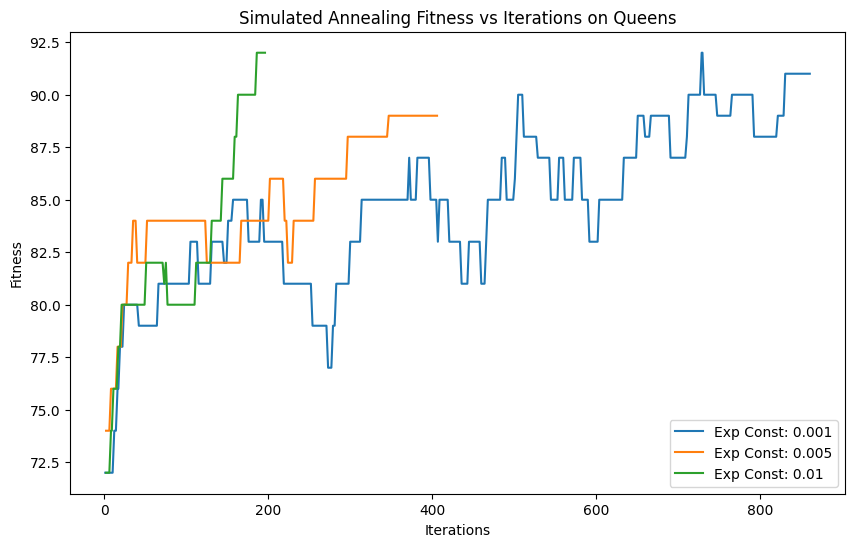
\includegraphics[width=\textwidth]{image/queens/sa.png}
        \caption{}
        \label{fig:queenssa}
    \end{subfigure}
    \vskip\baselineskip
    \begin{subfigure}[b]{0.49\textwidth}
        \centering
        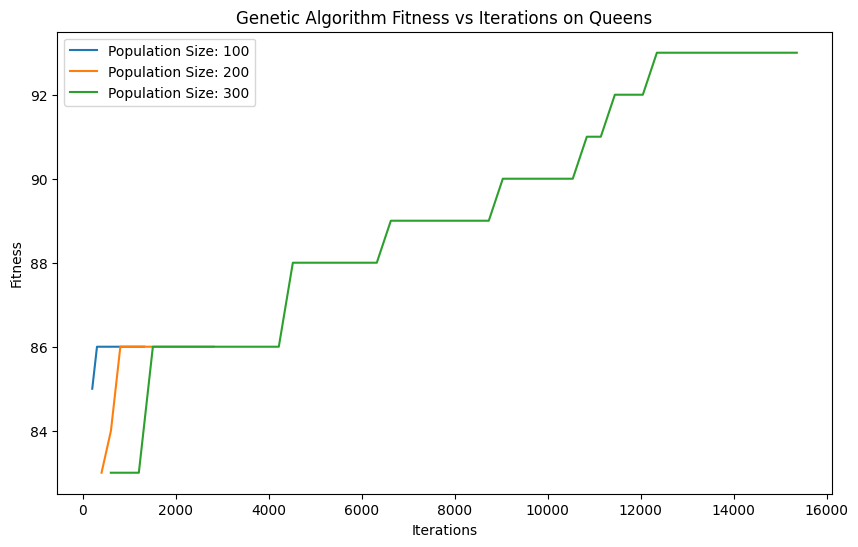
\includegraphics[width=\textwidth]{image/queens/ga.png}
        \caption{}
        \label{fig:queensga}
    \end{subfigure}
    \hfill
    \begin{subfigure}[b]{0.49\textwidth}
        \centering
        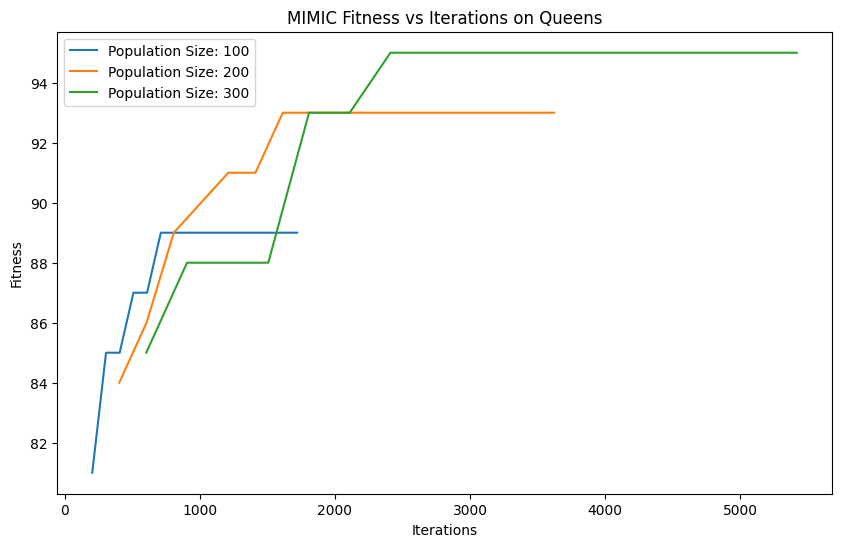
\includegraphics[width=\textwidth]{image/queens/mimic.png}
        \caption{}
        \label{fig:queensmimic}
    \end{subfigure}
    \caption{Fitness vs. iterations for the Queens Problem using different randomized optimization algorithms: (a) RHC, (b) SA, (c) GA, and (d) MIMIC. The plots show the impact of varying key parameters—restarts for RHC, exponential cooling for SA, population sizes for GA, and population sizes for MIMIC—on the fitness progression over iterations.}
    \label{fig:queensgrid}
\end{figure*}

\subsection{Combinatorial Problems}

%knapsack
In the Knapsack problem, where the goal is to maximize the value of selected items while staying within a weight limit, the results demonstrate how each algorithm handles the combinatorial complexity. Genetic Algorithms (GA) perform the best, with an average fitness of 172.2 for a population size of 200 (Table X). GA’s crossover and mutation operations help it efficiently explore the solution space, as seen in Figure 8(c), where the fitness improves steadily, demonstrating its capacity to balance exploration and exploitation effectively. MIMIC also shows strong performance, particularly with a population size of 100, achieving an average fitness of 162.0 (Table X). However, as shown in Figure 8(d), MIMIC's fitness progression tends to plateau after an initial steep climb, especially for larger population sizes, indicating that the algorithm struggles to continue improving beyond a certain point in this combinatorial context. Simulated Annealing (SA) performs moderately well, reaching an average fitness of 111.0 with an exponential constant of 0.001 (Table X). However, its performance fluctuates, as seen in Figure 8(b), where SA either converges rapidly or lags behind, depending on the cooling schedule, reflecting the difficulty of tuning SA for combinatorial problems. Randomized Hill Climbing (RHC) performs poorly compared to the other methods, with an average fitness of only 91.2 with 10 restarts, as shown in Table X and Figure 8(a). RHC’s inability to effectively escape local optima and explore larger portions of the solution space hampers its performance in the more complex search space of the Knapsack problem, a limitation that has been consistent across the other problems analyzed. This analysis reinforces the notion that algorithms like GA and MIMIC, which can handle larger and more complex search spaces, are better suited for combinatorial optimization tasks like Knapsack.
\begin{table*}[h!]
    \centering
    \caption{Knapsack Problem Results for RHC, SA, GA, and MIMIC with Different Hyperparameters}
    \begin{tabular}{|c|c|c|c|c|c|c|c|}
        \hline
        \textbf{Algorithm} & \textbf{Param} & \textbf{Run 1} & \textbf{Run 2} & \textbf{Run 3} & \textbf{Run 4} & \textbf{Average Fitness} & \textbf{Iterations} \\ \hline
        
        \textbf{RHC} & Restarts = 0 & 0.0 & 0.0 & 96.0 & 0.0 & 19.2 & 10 \\ \hline
        \textbf{RHC} & Restarts = 5 & 0.0 & 109.0 & 0.0 & 121.0 & 46.0 & 10 \\ \hline
        \textbf{RHC} & Restarts = 10 & 119.0 & 102.0 & 0.0 & 127.0 & 91.2 & 21 \\ \hline
        
        \textbf{SA} & ExpConst = 0.001 & 135.0 & 102.0 & 94.0 & 127.0 & 111.0 & 13 \\ \hline
        \textbf{SA} & ExpConst = 0.005 & 116.0 & 131.0 & 113.0 & 103.0 & 114.6 & 167 \\ \hline
        \textbf{SA} & ExpConst = 0.01 & 122.0 & 0.0 & 92.0 & 110.0 & 84.8 & 196 \\ \hline
        
        \textbf{GA} & PopSize = 100 & 162.0 & 173.0 & 170.0 & 172.0 & 167.4 & 37 \\ \hline
        \textbf{GA} & PopSize = 200 & 172.0 & 173.0 & 171.0 & 174.0 & 172.2 & 63 \\ \hline
        \textbf{GA} & PopSize = 300 & 176.0 & 175.0 & 176.0 & 176.0 & 175.8 & 46 \\ \hline
        
        \textbf{MIMIC} & PopSize = 100 & 162.0 & 128.0 & 131.0 & 133.0 & 145.0 & 28 \\ \hline
        \textbf{MIMIC} & PopSize = 200 & 132.0 & 136.0 & 127.0 & 127.0 & 129.8 & 15 \\ \hline
        \textbf{MIMIC} & PopSize = 300 & 136.0 & 137.0 & 136.0 & 139.0 & 136.8 & 18 \\ \hline
        
    \end{tabular}
    \label{tab:knapsack_results}
\end{table*}
\begin{figure*}[htbp]
    \centering
    \begin{subfigure}[b]{0.49\textwidth}
        \centering
        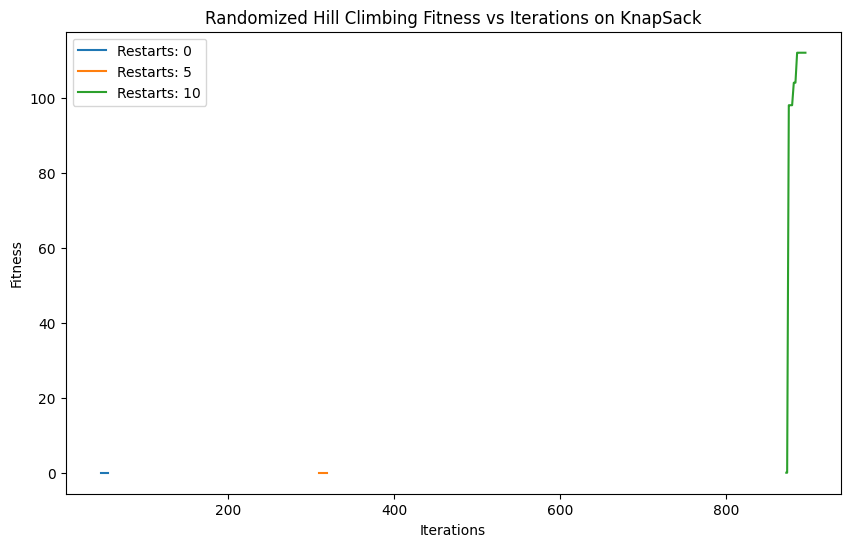
\includegraphics[width=\textwidth]{image/knapsack/rhc.png}
        \caption{}
        \label{fig:knapsackrhc}
    \end{subfigure}
    \hfill
    \begin{subfigure}[b]{0.49\textwidth}
        \centering
        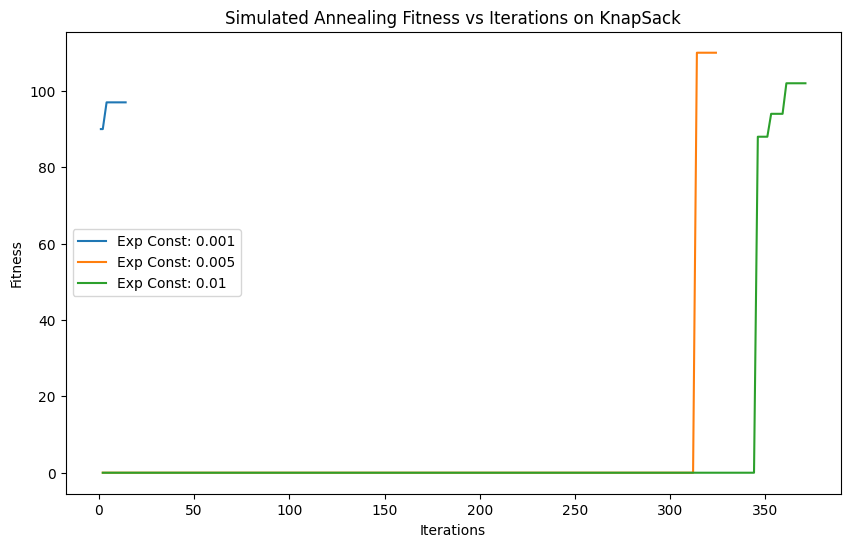
\includegraphics[width=\textwidth]{image/knapsack/sa.png}
        \caption{}
        \label{fig:knapsacksa}
    \end{subfigure}
    \vskip\baselineskip
    \begin{subfigure}[b]{0.49\textwidth}
        \centering
        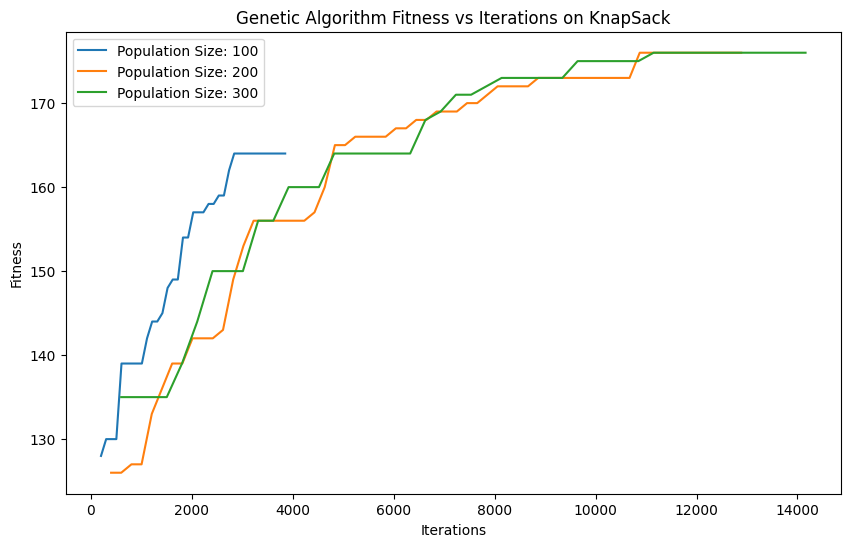
\includegraphics[width=\textwidth]{image/knapsack/ga.png}
        \caption{}
        \label{fig:knapsackga}
    \end{subfigure}
    \hfill
    \begin{subfigure}[b]{0.49\textwidth}
        \centering
        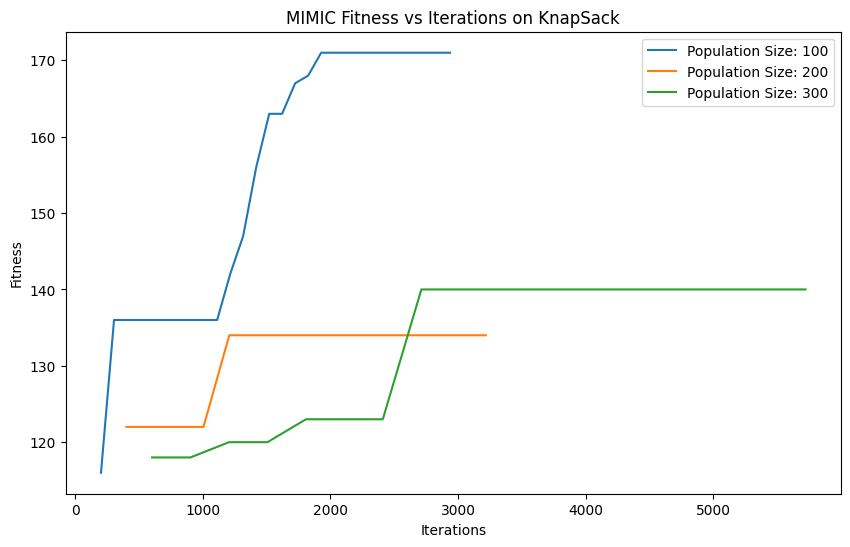
\includegraphics[width=\textwidth]{image/knapsack/mimic.png}
        \caption{}
        \label{fig:knapsackmimic}
    \end{subfigure}
    \caption{Fitness vs. iterations for the Knapsack Problem using different randomized optimization algorithms: (a) RHC, (b) SA, (c) GA, and (d) MIMIC. The plots show the impact of varying key parameters—restarts for RHC, exponential cooling for SA, population sizes for GA, and population sizes for MIMIC—on the fitness progression over iterations.}
    \label{fig:knapsackgrid}
\end{figure*}

%Across groups summary
\subsection{Cross-Group Performance Analysis of Optimization Algorithms}
In comparing the performance of Randomized Hill Climbing (RHC), Simulated Annealing (SA), Genetic Algorithms (GA), and MIMIC across binary, permutation, and combinatorial problem groups, distinct trends in efficiency, computational cost, and solution quality emerge. As seen in Fig. 10, MIMIC and GA perform exceptionally well across all problem groups, particularly excelling in the combinatorial group, where MIMIC achieved over 80\% of the total possible fitness for the Knapsack problem, and GA reached 86\%. For the permutation group, MIMIC showed a similar trend with fitness values hovering around 90\% in problems like Queens, while GA exhibited consistent, though slightly slower, performance. The binary group had a simpler fitness landscape, allowing both MIMIC and GA to converge efficiently, although the binary problems generally presented fewer local optima and required less sophisticated search mechanisms than the combinatorial and permutation problems.

However, a deeper comparison reveals trade-offs between solution quality and computational costs. As shown in Fig. 9, MIMIC incurs higher computational cost in terms of wall clock time across all groups, particularly in the permutation and combinatorial problems. For example, in the binary problem group, MIMIC's higher wall clock time was more pronounced compared to GA, which maintained moderate time efficiency while still producing competitive fitness results. This highlights MIMIC’s strength in consistently achieving high solution quality, albeit at the cost of increased computation, making it more suitable for cases where accuracy is paramount, and computational resources are less constrained. On the other hand, GA demonstrated a more balanced approach across groups, achieving high-quality solutions with significantly lower computational overhead than MIMIC, making it more appropriate for situations where a compromise between solution quality and time efficiency is needed.

RHC and SA, as expected, struggled to maintain competitive performance across the groups. As shown in Fig. 11, SA required the highest number of iterations, particularly in binary and permutation problems, reflecting its difficulty in efficiently exploring simpler landscapes where local optima are less challenging to escape. While SA did perform reasonably well in more complex combinatorial problems like Knapsack, its high iteration count and instability in convergence make it less suitable than GA or MIMIC for large-scale optimization tasks. RHC consistently underperformed, achieving less than 60\% of the total possible fitness in all groups, with its performance particularly poor in the combinatorial problems. Its inability to explore the search space effectively and its susceptibility to getting trapped in local optima, as shown by the relatively few iterations in Fig. 11, make it the least effective algorithm across all problem types.
\begin{figure}[h!]
    \centering
    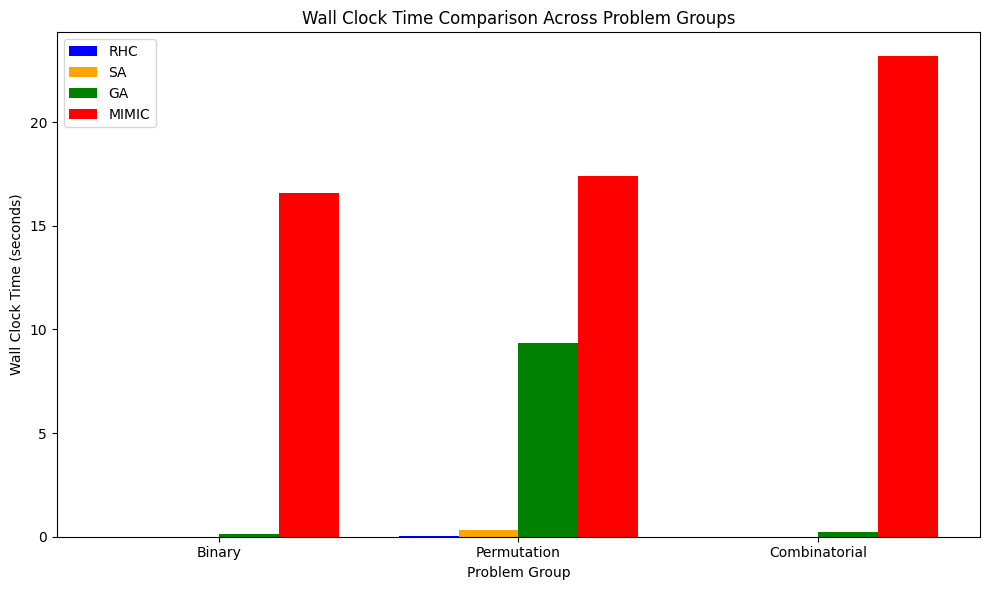
\includegraphics[width=0.46\textwidth]{image/timeplot.png}
    \caption{Wall Clock Time Comparison Across Problem Groups (Binary, Permutation, Combinatorial) for RHC, SA, GA, and MIMIC}
    \label{fig:wall_clock_time_comparison}
\end{figure}

\begin{figure}[h!]
    \centering
    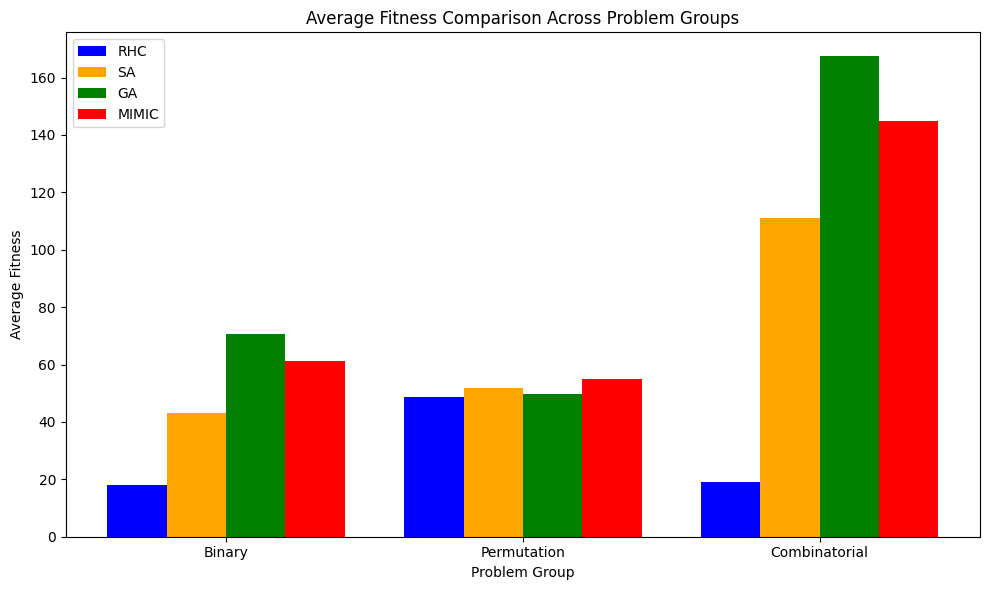
\includegraphics[width=0.46\textwidth]{image/fitplot.png}
    \caption{Average Fitness Comparison Across Problem Groups (Binary, Permutation, Combinatorial) for RHC, SA, GA, and MIMIC}
    \label{fig:average_fitness_comparison}
\end{figure}

\begin{figure}[h!]
    \centering
    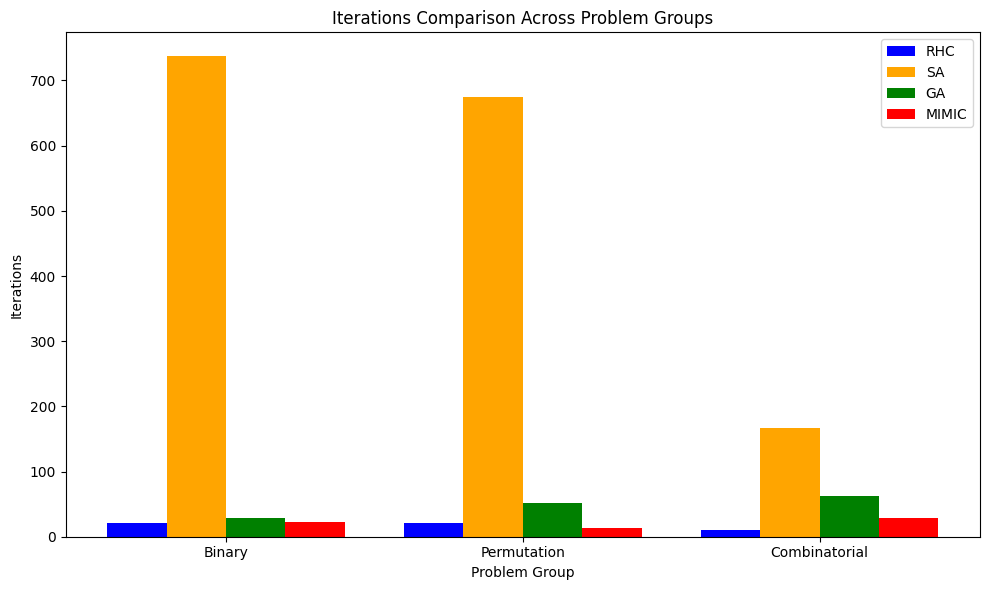
\includegraphics[width=0.46\textwidth]{image/iterplot.png}
    \caption{Iterations Comparison Across Problem Groups (Binary, Permutation, Combinatorial) for RHC, SA, GA, and MIMIC}
    \label{fig:iterations_comparison}
\end{figure}

\begin{table*}[h!]
\centering
\caption{Algorithm selection based on problem group, fitness achieved, and computational cost.}
\begin{tabular}{|p{2cm}|p{1cm}|p{2cm}|p{2cm}|p{4cm}|p{4cm}|}
\hline
\textbf{Problem Group}       & \textbf{Best Algorithm} & \textbf{Fitness Achieved (\% of Optimum)} & \textbf{Computational Cost (Time/Iterations)} & \textbf{When to Use}                                                                                       & \textbf{Trade-offs}                                                                                               \\ \hline
\textbf{Binary}              & GA, MIMIC               & 90-95\%                                    & Moderate (GA), High (MIMIC)                    & Use GA for most binary problems due to its lower time cost, MIMIC when accuracy is critical                  & MIMIC gives slightly better fitness, but GA is faster overall                                                      \\ \hline
\textbf{Permutation}         & MIMIC, GA               & 85-90\%                                    & High (MIMIC), Moderate (GA)                    & Use MIMIC for complex problems like Queens where interdependencies are important, GA for faster convergence  & MIMIC provides better solutions but at significantly higher computational cost                                     \\ \hline
\textbf{Combinatorial}       & GA                      & 85-90\%                                    & Moderate                                       & Use GA for large combinatorial problems with complex constraints                                             & MIMIC can be used for very high accuracy but at a significant computational trade-off in terms of time             \\ \hline
\textbf{Low Computational Cost} & RHC                   & \textless{}60\%                            & Low                                            & Use RHC only when computation resources are limited and solution quality is not critical                     & Very poor solution quality makes RHC unsuitable for most large or complex problems                                 \\ \hline
\textbf{High Accuracy Need}  & MIMIC                   & 85-95\%                                    & High                                           & Use MIMIC when solution quality is the highest priority, regardless of computational cost                    & High computational cost, particularly in larger and more complex problem types                                     \\ \hline
\end{tabular}
\end{table*}
\section{conclusion}
In this study, we assessed the performance of four optimization algorithms—Randomized Hill Climbing (RHC), Simulated Annealing (SA), Genetic Algorithms (GA), and MIMIC—by analyzing their underlying mechanisms and comparing their strengths and weaknesses. These algorithms were tested across three distinct problem categories: binary (including OneMax, FlipFlop, FourPeaks, SixPeaks, and ContinuousPeaks), permutation (Traveling Salesman and N-Queens), and combinatorial (Knapsack). The performance and behavior of each algorithm were evaluated through multiple experimental trials. Results showed that while MIMIC and GA demonstrated superior performance, they also came with significantly higher computational costs. Ongoing research aims to develop more efficient algorithms that maintain high performance while reducing computational overhead

\section*{Funding}
This research is supported by the Natural Sciences and Engineering Research Council of Canada (NSERC) Collaborative Research and Training Experience (CREATE) program, grant number: 565429-2022.

\section*{Data Availability Statement}
The data generated during the course of this study are available on GitHub at \url{https://github.com/semtu/On-Automated-Object-Grasping-for-Intelligent-Prosthetic-Hands-Using-Machine-Learning}.

\section*{Conflicts of Interest}
The authors declare no conflicts of interest.

\bibliographystyle{plain}
\bibliography{references}
\end{document}

